%% HARNESS-Review — ACM Computing Surveys manuscript (acmart).
%% Overleaf: link this GitHub repo (Menu > GitHub) and set main.tex as the root document.
%% For TMLR, compile main_tmlr.tex instead (same sections/ and references/).
\documentclass[manuscript,screen,review]{acmart}
\usepackage{booktabs}
\usepackage{graphicx}
\usepackage{xcolor}
\usepackage{colortbl}   % subtle best-value shading in results tables (writing standard, section 3)
%% RQ3 numbers are generated from the analysis outputs (make_rq3_tables in the replication
%% package) as macros and loaded here, so every section, not only section 7, can cite them.
% RQ3 prose macros (text-mode safe; *Pct macros are bare numbers)
% GENERATED by scripts/make_rq3_tables.py - do not edit; re-run the script instead.
% sources (mtime, UTC):
%   data/analysis/ablation_summary_corpus.json  (2026-09-28T13:53:56Z)
%   data/analysis/ablation_pooled_corpus.csv  (2026-09-28T13:53:56Z)
%   data/analysis/ablation_credible_corpus.csv  (2026-09-28T13:53:56Z)
%   data/analysis/ablation_bias_corpus.csv  (2026-09-28T13:53:56Z)
%   data/analysis/ablation_contrasts_corpus.csv  (2026-09-28T13:53:56Z)
%   data/analysis/ablation_coverage_summary.json  (2026-09-25T16:01:11Z)
%   data/analysis/ablation_coverage_summary_corpus.json  (2026-09-28T13:53:57Z)
%   schema/dimensions.json  (2026-09-25T14:21:14Z)
%   paper/tables/outcomes_summary.json  (2026-09-25T15:27:23Z)
%   data/results.csv  (2026-09-24T23:51:08Z)
%   data/systems.json  (2026-09-25T10:17:13Z)
%   data/analysis/corpus_ablation_rows.csv  (live; rows of the pooled snapshot's papers only)
%   data/analysis/corpus_ablation_outcomes.csv  (live; rows of the pooled snapshot's papers only)
% generated: 2026-09-28T13:53:57Z
% papers the corpus-wide harvest has read (snapshot pooled)
\newcommand{\rqCorpusPapersExtracted}{2{,}824}
% corpus-harvest papers contributing >=1 pooled contrast (after de-duplication)
\newcommand{\rqCorpusPapersWithContrast}{1{,}264}
% corpus-harvest contrasts pooled (after de-duplication against the coded set)
\newcommand{\rqCorpusContrasts}{5{,}928}
% coded-set harvest contrasts
\newcommand{\rqCodedContrasts}{75}
% coded-set harvest papers
\newcommand{\rqCodedPapers}{42}
% all contrasts pooled, coded-set + corpus
\newcommand{\rqTotalContrasts}{6{,}003}
% distinct papers behind them
\newcommand{\rqTotalPapers}{1{,}278}
% corpus contrasts dropped as already in the coded-set harvest
\newcommand{\rqCorpusDuplicatesDropped}{48}
% dimensions pooled (>= rqMinPapers papers)
\newcommand{\rqPoolableDims}{22}
% papers needed to pool a dimension
\newcommand{\rqMinPapers}{3}
% bare number: % of contrasts favouring the component, coded-set + corpus, over the pooled (bias-diagnosed) dimensions, contrast-weighted
\newcommand{\rqSignSharePct}{90.0}
% pooled dimensions whose 95% prediction interval includes zero
\newcommand{\rqPIIncludesZeroCount}{22}
% pooled dimensions whose prediction interval excludes zero
\newcommand{\rqPIExcludesZeroDims}{none}
% lower prediction-interval bound of each of those dimensions
\newcommand{\rqPIExcludesZeroLower}{none}
% pooled dimensions surviving the bias discount on the z interval
\newcommand{\rqDiscountSurviveZ}{14}
% ... on the Hartung-Knapp interval
\newcommand{\rqDiscountSurviveHK}{14}
% min to max DL pooled effect over the dimensions surviving on z
\newcommand{\rqEffectRangeSurviving}{\ensuremath{+0.114} to \ensuremath{+0.259}}
% first to third quartile of those effects (inclusive quartiles)
\newcommand{\rqEffectIQRSurviving}{\ensuremath{+0.159} to \ensuremath{+0.188}}
% bare number: median per-dimension publication-bias discount, %
\newcommand{\rqMedianDiscountPct}{49.5}
% dimensions with Egger p < 0.1, intercept sign in parentheses
\newcommand{\rqEggerFlaggedDims}{observation\_format (\ensuremath{-}), tool\_count (\ensuremath{-}), planning\_granularity (\ensuremath{-}), long\_term\_memory (\ensuremath{-}), self\_verification (\ensuremath{-}), termination\_condition (\ensuremath{+})}
% focal dimension: papers
\newcommand{\rqSVPapers}{525}
% focal dimension: contrasts
\newcommand{\rqSVContrasts}{1{,}687}
% focal dimension: DL pooled effect
\newcommand{\rqSVPooled}{\ensuremath{+0.152}}
% focal dimension: discounted effect
\newcommand{\rqSVDiscounted}{\ensuremath{+0.152}}
% focal dimension: 95% prediction interval, with brackets
\newcommand{\rqSVPI}{\ensuremath{[-0.798, +1.101]}}
% focal dimension: 95% z confidence interval, with brackets
\newcommand{\rqSVCIz}{\ensuremath{[+0.109, +0.194]}}
% focal dimension: 95% Hartung-Knapp interval, with brackets
\newcommand{\rqSVCIHK}{\ensuremath{[+0.128, +0.175]}}
% Spearman rho, layer silence vs corpus-wide ablation density
\newcommand{\rqCoverageRho}{\ensuremath{-0.738}}
% its exact one-sided permutation p
\newcommand{\rqCoverageP}{0.023}
% the same rho on the coded-set harvest only
\newcommand{\rqCodedCoverageRho}{\ensuremath{-0.854}}
% its exact p
\newcommand{\rqCodedCoverageP}{0.0065}
% ablatable dimensions with no contrast at all
\newcommand{\rqZeroDimCount}{7}
% ablatable dimensions (layers A-H)
\newcommand{\rqAblatableDimCount}{31}
% those dimensions
\newcommand{\rqZeroDimList}{cost controls (F2), evaluation hooks (H3), execution isolation (G1), filesystem access (G2), network policy (G3), permission model (G4) and replayability (H2)}
% layers with no ablated dimension ('empty' if none)
\newcommand{\rqZeroLayerList}{G (sandbox and environment)}
% every F/G/H dimension with >=1 contrast: key (papers/contrasts), corpus-wide
\newcommand{\rqFGHPaperCounts}{termination\_condition (9/28), timeouts (1/1), tracing (4/10), guardrails (21/37)}
% noun phrase: share of each prefilter tier the harvest has read
\newcommand{\rqHarvestTierCoverage}{96.7\% of the top-signal tier and 90.1\% of the second}
% papers in the top-signal tier
\newcommand{\rqHarvestTopTierPapers}{899}
% papers in the second tier
\newcommand{\rqHarvestSecondTierPapers}{2{,}170}
% date of the harvest snapshot pooled
\newcommand{\rqHarvestDate}{28 September 2026}
% contrasts on the pooled dimensions: the denominator of rqSignSharePct
\newcommand{\rqSignDenom}{6{,}001}
% of those, contrasts whose metric names its direction (higher / lower is better)
\newcommand{\rqPolarityStatedN}{4{,}080}
% of those, favouring the component
\newcommand{\rqPolarityStatedFavour}{3{,}701}
% bare number: their share favouring the component, %
\newcommand{\rqPolarityStatedFavourPct}{90.7}
% contrasts whose metric names no direction: higher-is-better assumed
\newcommand{\rqPolarityAssumedN}{1{,}921}
% of those, favouring the component
\newcommand{\rqPolarityAssumedFavour}{1{,}700}
% bare number: their share favouring the component, %
\newcommand{\rqPolarityAssumedFavourPct}{88.5}
% contrasts whose variance is a flat assumed relative SE, not a binomial reconstruction
\newcommand{\rqVarAssumedN}{2{,}857}
% Spearman rho, silence vs density, with the seven classification rules undone
\newcommand{\rqPreRuleRho}{\ensuremath{-0.738}}
% its exact one-sided permutation p
\newcommand{\rqPreRuleP}{0.023}
% sandbox-layer (G) contrasts before the rules; after them there are none
\newcommand{\rqPreRuleGContrasts}{20}
% of those, reassigned by a rule to the dimension the removal takes away
\newcommand{\rqPreRuleGRemapped}{13}
% of those, dropped by a rule: delta_metric_as_score 2, scores_not_separable 4, tool_gating_is_tool_interface 1
\newcommand{\rqPreRuleGDropped}{7}
% rows the label-contradicts-orientation rule dropped, on pooled dimensions
\newcommand{\rqDCLDropped}{169}
% of those, rows that do not favour the component as the extraction stage oriented them
\newcommand{\rqDCLAgainst}{71}
% bare number: the sign share had those rows been kept as the extraction oriented them
\newcommand{\rqSignShareWithDCLPct}{89.1}
% headline keys whose reference side is only recurring baseline harnesses
\newcommand{\rqXPBaselineKeys}{7}
% the headline's remaining keys
\newcommand{\rqXPOtherKeys}{11}
% the headline effect on those keys, within-key sd
\newcommand{\rqXPOtherEffect}{\ensuremath{+0.57}}
% its 95% bootstrap interval over keys, with brackets
\newcommand{\rqXPOtherCI}{\ensuremath{[-0.19, +1.23]}}
% its two-sided within-key permutation p
\newcommand{\rqXPOtherP}{0.129}

\graphicspath{{figures/}}

\acmJournal{CSUR}
\citestyle{acmauthoryear}

\title{The Anatomy of Agent Harnesses: A Systematic Review, Unified Taxonomy, and Coded Dataset (HARNESS-DB) of LLM Agent Scaffolding, 2022--2026}

\author{Bhaskar Gurram}
\email{gurrambhaskar.ai@gmail.com}
\affiliation{%
  \institution{Independent researcher}
  \country{USA}}

\begin{document}

\begin{abstract}
% Abstract text goes here (no \section).
We conduct the first PRISMA-grade systematic review of LLM agent harnesses (October 2022 to August 2026), reconcile prior harness taxonomies into a unified schema, release HARNESS-DB, and report a corpus-wide quantitative synthesis of harness design choices against reported task success and cost.

\end{abstract}

\begin{CCSXML}
<ccs2012>
 <concept><concept_id>10010147.10010178</concept_id><concept_desc>Computing methodologies~Artificial intelligence</concept_desc><concept_significance>500</concept_significance></concept>
 <concept><concept_id>10011007.10011074</concept_id><concept_desc>Software and its engineering~Software creation and management</concept_desc><concept_significance>300</concept_significance></concept>
</ccs2012>
\end{CCSXML}
\ccsdesc[500]{Computing methodologies~Artificial intelligence}
\ccsdesc[300]{Software and its engineering~Software creation and management}
\keywords{LLM agents, agent harness, agent scaffolding, systematic review, taxonomy, dataset}

\maketitle

\section{Introduction}
\label{sec:intro}

An LLM agent's behavior is set as much by its harness as by its model. The harness is the software
layer that assembles the model's input at every step, executes the actions the model selects, and
decides whether to continue; it also holds state, verifies output, bounds cost, isolates execution,
and records what happened. Hold the model fixed and change the harness, and the reported score moves
\citep{guo2026qa2task}, so an agent comparison that does not disclose its harness cannot be
interpreted \citep{zhang2026harnessreporting}. The design question is how harnesses are built and
which design choices change outcomes.

Seven prior surveys and taxonomies address harnesses, and none can answer that question.
\citet{guo2026qa2task} decompose the harness into six runtime responsibilities and alone compile
same-model, different-harness leaderboard evidence, but the harness enters that evidence as a name
rather than as coded design. \citet{rombaut2026insidescaffold} reads the source of thirteen coding
agents with a file and line behind every claim, and \citet{barbaste2026anatomy} read the source of
eleven harnesses at pinned releases.
\citet{li2026harnessengineering}, \citet{meng2026harnesssurvey}, \citet{zhong2026responsibilities},
and \citet{harnesscategorical2026} contribute a layered taxonomy, a formal component tuple, a maturity
ladder, and a categorical semantics. Four technical limits are shared. First, none samples from an
enumerated frame of released systems, so none can estimate how far its well-known systems depart from
the population. Second, none codes design with re-openable evidence per cell beyond thirteen systems,
so a claimed value cannot be rechecked against its source. Third, none was registered before coding
or reports agreement per dimension, and \citet{li2026harnessengineering} state that they do not report
Cohen's kappa; without a reliability gate, consistent use of a category is assumed rather than shown.
Fourth, none records documented silence as a state of its own, so where the evidence is documents
rather than code, an undocumented component and an absent one receive the same mark. A catalog built
this way says what exists and what to call it; it cannot measure what the field discloses or relate
design to outcome.

We address the design question with a review registered on OSF (\texttt{osf.io/ab2wn}) before coding
and reported under PRISMA 2020 \citep{page2021prisma}, built from three frameworks
(Figure~\ref{fig:pipeline}). \emph{Two-Tier Escalation Screening} settles each retrieved record at
title and abstract where it can and escalates the rest to a full-text reading of paper, repository,
and documentation together. Grouping the included records into systems gives a sampling frame of
6,504 harnesses, sampled by stratum and weighted back. \emph{Evidence-Anchored Coding} codes 1,256
systems on 38 dimensions in nine layers with a verbatim quote and a re-openable locator behind every
claimed value. Before the schema froze, each dimension was tested against a floor of
$\kappa \ge 0.6$ on a double-coded sample. The \emph{Three-State Cell Contract} gives every cell
exactly one state: a value, \texttt{not\_reported} when the sources were read and are silent, or
\texttt{unresolved} when the cell could not be settled, so silence is counted and never rounded to
absence. This is not the first survey of agent harnesses. To our knowledge, it is the first
pre-registered review of the area to report per-dimension coding reliability, and the first to analyze
reported outcomes against coded design dimensions rather than harness identity.

\begin{figure}[t]
  \centering
  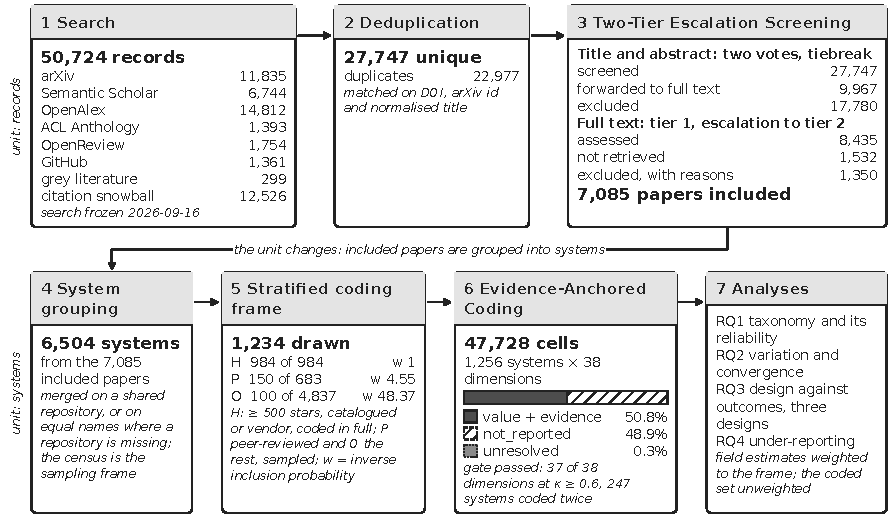
\includegraphics[width=\linewidth]{pipeline_overview}
  \caption{The study at a glance. Two-Tier Escalation Screening takes 27,747 screened records to a
  frame of 6,504 systems; Evidence-Anchored Coding turns 1,256 of them into 47,728 cells under the
  Three-State Cell Contract.}
  \label{fig:pipeline}
\end{figure}

The results say that the literature describes what a harness is and not what bounds it, and that its
outcome evidence cannot yet say which design choices matter. Of the 47,728 cells, 48.9\% record
documented silence, and the silence concentrates in the layers that govern safe deployment. Beneath a
comparability ceiling of 53 of 1,256 coded systems (4.2\%), of the two design estimates that survive, one is an
upper bound and the other is biased in both directions.

Four registered questions organize the paper.

\begin{enumerate}
  \item[\textbf{RQ1}] What are a harness's structural components, and can a taxonomy of them be applied
  at $\kappa \ge 0.6$ per dimension?
  \item[\textbf{RQ2}] How do design choices vary across systems, and how did that variation move
  between 2022 and 2026?
  \item[\textbf{RQ3}] Which design choices are associated with reported success, cost, or robustness,
  with benchmark and base model held constant?
  \item[\textbf{RQ4}] Which dimensions does the literature systematically fail to report?
\end{enumerate}

Our contributions follow.

\begin{enumerate}
  \item \textbf{An evidence-anchored release (RQ1).} HARNESS-DB releases every coded value with its evidence,
  at mean per-dimension Cohen's kappa 0.784 [0.765, 0.800] over 247 double-coded systems (37 of 38
  dimensions at or above 0.6; four intervals include the floor), which measures reproducibility, not
  correctness.

  \item \textbf{A weighting inversion (RQ2).} Repository-primary systems are 69.2\% of 1,252 coded
  systems carrying a value but an estimated 33.3\% of the frame, so a sample of well-known systems
  reverses the modal release artifact.

  \item \textbf{An under-reporting gradient (RQ4).} The weighted \texttt{not\_reported} rate runs from
  24.9\% $\pm$ 1.2 in the control-loop layer to 81.6\% $\pm$ 1.8 in the sandbox layer, a statement
  about documents, not about systems.

  \item \textbf{A measured trap (RQ2).} Mean corrected Cram\'er's V is 0.167, and treating silence as a
  category raises significant pairs from 385 to 648 of 666, 265 of them significant only when silence
  is a level.

  \item \textbf{A registered negative and a diversification (RQ2).} Clustering fails its silhouette
  floor, 0.120 against 0.25 (verdict negative); in the coded set, 10 of 34 dimensions show a diversity
  change whose interval
  excludes zero against 1.7 expected under the global null, of which 9 survive Benjamini--Hochberg
  (6 diversified, 3 converged).

  \item \textbf{A comparability ceiling and a selection-sensitive association (RQ3).} With 53 of 1,256 systems
  comparable to any peer, the registered regression was not fitted, and multi-agent topology is associated
  with $+0.88$ within-key standard deviations [$+0.38$, $+1.31$]. Drift attenuates it, but the choice of
  reference systems can inflate it: on the \rqXPOtherKeys{} keys whose references are not all recurring
  baselines the estimate is \rqXPOtherEffect{} \rqXPOtherCI{}, so the net direction of bias is unknown.

  \item \textbf{An upper bound that does not discriminate (RQ3).} On the completed corpus-wide harvest of
  authors' own ablations, which read \rqHarvestTierCoverage, \rqDiscountSurviveZ{} of
  \rqPoolableDims{} poolable dimensions pass the bias-discount rule with pooled relative gains of
  \rqEffectRangeSurviving{} (middle half \rqEffectIQRSurviving) before a median discount of \rqMedianDiscountPct\%, each an upper bound,
  and \rqSignSharePct\% of contrasts favour the ablated component: these ablations barely separate design
  dimensions. Self-verification, which the coded-set harvest singled out, is worth at most about
  \rqSVDiscounted{} relative; our compute-matched test of it failed its pilot band, and in 56
  diagnostic runs model-written self-checks accepted the first attempt 50 times, and 41 of 48 in a
  second pilot.

  \item \textbf{An evidence gap (RQ3).} On the coded-set harvest none of the eleven dimensions of
  layers F, G, and H carried a published ablation. The corpus-wide harvest reaches four of them,
  through 1 to 21 papers each; of the \rqPreRuleGContrasts{} contrasts it first attributed to layer G,
  \rqPreRuleGRemapped{} removed code-execution feedback or file-system tools and the other
  \rqPreRuleGDropped{} were unreadable or named no sandbox mechanism, and under the fixed mapping rules \rqZeroDimCount{} of
  \rqAblatableDimCount{} ablatable dimensions, all four of layer G among them, carry none. Ablation
  density falls as silence rises (Spearman's $\rho$ of \rqCoverageRho, exact one-sided permutation $p$
  of \rqCoverageP), an absence of evidence, not evidence that those components do not matter.
\end{enumerate}

\section{Background and definition}
\label{sec:background}

\subsection{What a harness is}
\label{subsec:definition}

An agent harness is the software layer between a language model and a task environment that
repeatedly assembles the model's input, executes the model's chosen actions, and decides whether to
continue. Let $M$ be a model, a map from input to output tokens together with its decoding
configuration, and let $E$ be a task environment: a state space, executable operations with observable
results, and a task specification. $M$ cannot act on $E$ and $E$ cannot read $M$; the harness $H$
connects them by implementing eight functions. It (i) assembles input, (ii) exposes and executes
actions, (iii) decides continuation and termination, (iv) holds state beyond one model call,
(v) verifies and repairs, (vi) enforces budgets and permissions, (vii) isolates execution, and
(viii) records and governs what happened. An agent is the run-time triple $(M, H, E)$, which makes the
harness effect well posed: hold $M$ and $E$ fixed and vary $H$.

Clauses (i) to (iii) are necessary; without them a layer is a prompt, a tool server, or a pipeline.
Clauses (iv) to (viii) may be trivial, and a trivial value is still a value: a harness that runs the
model in the host process is coded \texttt{none} on execution isolation, not \texttt{not\_reported}.
The minimal harness formats the transcript, executes one parsed action, and stops on a finish action
or a step cap; ReAct \citep{yao2023react} is exactly that, and is the earliest system in the corpus.
Later systems elaborate particular clauses. Reflexion keeps verbal reflections on task feedback in an
episodic memory \citep{shinn2023reflexion}, and CodeAct makes executable Python code the action space
\citep{wang2024codeact}. AutoGen and MetaGPT run several agents that converse or hold assigned roles
\citep{wu2023autogen,hong2023metagpt}, and Agent S and OS-Copilot act through a computer's interface,
evaluated on OSWorld and GAIA \citep{agashe2024agents,wu2024oscopilot,xie2024osworld,mialon2023gaia}.
The unit of analysis is the system, not the paper: coding papers would count a popular harness once
per publication and a harness with no paper not at all.

One test decides every boundary case: whether changing the thing in question, with everything else
fixed, would change what the model sees, what it can do, or when it stops. Table~\ref{tab:boundary} applies
it where the definition is most often probed. The pattern is that a part is not a system, while the
loop a framework or benchmark ships is one.

\begin{table}[t]
  \caption{Boundary cases and how the definition decides them.}
  \label{tab:boundary}
  \footnotesize
  \begin{tabular}{@{}p{0.40\linewidth}p{0.29\linewidth}p{0.25\linewidth}@{}}
    \toprule
    Case & Decision & Reason \\
    \midrule
    Weights, decoding settings, trained call syntax & Model, not harness & Fixed inside a forward
    pass \\
    Tool schemas, output parser, re-prompts & Harness & Change what the model sees \\
    Reasoning model that stops thinking itself & Harness still owns (iii) & Harness decides on
    another call \\
    \midrule
    Prompt; chain-of-thought with self-consistency; tree of thoughts \citep{yao2023tot} & Not a system & No action on an environment \\
    ReAct \citep{yao2023react} & System & Parse, execute, append, repeat \\
    SWE-agent with GPT-4 on SWE-bench Lite & An agent; SWE-agent is the system
    \citep{yang2024sweagent} & An agent is $(M, H, E)$ \\
    \midrule
    Framework library, e.g.\ LangGraph \citep{langgraph} or CrewAI \citep{crewai} & Coded via its default agent &
    A kit, not a loop \\
    Container the harness launches \citep{wang2024openhands} & Part of the harness & The harness
    configures it \\
    Sandbox product, protocol server, vector store, tracer & Not a system & One clause, not the
    loop \\
    \midrule
    Non-looping benchmark baseline \citep{jimenez2024swebench} & Not a system & It is $E$ \\
    Looping benchmark baseline \citep{zhou2023webarena,xie2024osworld,yao2024taubench,chezelles2024browsergym} & System & Loops a model over $E$ \\
    Tool-use fine-tuning \citep{schick2023toolformer} & Out of scope unless it adds a loop &
    Changes $M$, not $H$ \\
    Closed vendor product \citep{claudecode} & System if codable from documents & Defined by
    behavior \\
    \bottomrule
  \end{tabular}
\end{table}

\subsection{The nine layers}
\label{subsec:layers}

The eight clauses map onto coding layers A to H, plus a metadata layer M, for 38 dimensions.
Context assembly (A, four dimensions) governs what the model sees at each step, and tool interface
(B, five) what it may do and in what syntax. Control loop (C, five) governs what happens after a
step, including topology, delegation, and human checkpoints. Memory and state (D, three) covers what
persists within and across runs, verification and repair (E, three) whether an oracle checks the work,
and budget and termination (F, three) step, cost, and time bounds. Sandbox and environment (G, four)
covers isolation, filesystem, network, and permissions; observability and governance (H, four) covers
tracing, replay, evaluation hooks, and guardrails. Layer M (seven) describes the system record, such
as domain, openness, and primary artifact, and is excluded wherever a claim is about design. Three
placements are deliberate. Termination sits in F rather than C so that termination and budget are
counted together. Filesystem access and network policy sit apart from isolation because released
systems configure them independently. Observability and governance share H because in this corpus
they are reported together or not at all.

\subsection{The Three-State Cell Contract}
\label{subsec:cellstates}

The paper's measurement vocabulary is the Three-State Cell Contract. A cell is one system against one
dimension and holds exactly one state. A \emph{value} is backed by a verbatim quote and a re-openable
locator, and includes an absence found where the feature would be declared (50.8\% of the 47,728
cells). \texttt{not\_reported} means the sources were read and are silent (48.9\%), and
\texttt{unresolved} means the cell could not be settled (0.3\%). Silence is data about documents,
never absence in a system: the sources are silent on network policy for an estimated 93.3\% of
systems, which does not mean that 93.3\% of systems lack one. An \texttt{unresolved} cell is an
admission about our coding, excluded from every denominator and never pooled with
\texttt{not\_reported}, because pooling would inflate the silence rate by exactly what we failed to
code. Every share is labeled weighted, describing the frame, or unweighted, describing the coded set,
and carries its denominator. Section~\ref{sec:methods} gives the coding rule that enforces the
contract.

\section{Related work and the taxonomy crosswalk}
\label{sec:related}

Seven prior works give the agent harness a structure, and they divide by what they measure.
Catalogues and completeness matrices list systems against a scheme, taxonomies derive a scheme from a
few systems read closely, and outcome studies compare harnesses by name. The closest to our design
question (RQ3) is \citet{guo2026qa2task}. Each group is limited for our purpose by a mechanism, not by
incompleteness.

\paragraph{Broader surveys of LLM agents}
Beyond these seven, surveys of LLM agents organize the field by agent component or method rather than
by harness. \citet{wang2023agentsurvey} propose a unified framework for constructing agents and review
applications and evaluation strategies, and \citet{xi2023riseagents} divide an agent into brain,
perception, and action. Later surveys decompose agents into components and orchestration patterns
\citep{agenticai2026taxonomies,agentsystems2026survey}, classify reasoning frameworks as single-agent,
tool-based, or multi-agent \citep{agenticreasoning2025survey}, treat workflows as computation graphs
fixed before or during a run \citep{workflowopt2026survey}, and frame post-training, memory, and skills
as adaptation of an agent or its tools \citep{adaptation2025survey}. Others cover one domain, software
engineering \citep{seagentic2025survey} or deep research \citep{deepresearch2025agents}, or one
artifact: \citet{agenticframeworks2025} compare seven frameworks, among them CrewAI, LangGraph, and
AutoGen, and \citet{skills2026lifecycle} reads a 124-paper audit set on skill libraries, assembled by
snowballing rather than a PRISMA-style query. The unit in these surveys is a paper, method, or
framework, not a sampled population of released systems, and none reports an inter-coder agreement
statistic. Outside the survey literature, \citet{frameworksfallshort2026} classify 5,669 bug reports
from five agent frameworks and find that 76.00\% manifest as incorrect functionality.

\paragraph{Catalogues and completeness matrices}
These works estimate what the field contains. \citet{li2026harnessengineering} apply the seven-layer
ETCLOVG taxonomy to a public catalogue of 171 entries at its 2026-05-08 snapshot (368 at our last
check), assigning one primary layer to each of 138 artifacts. The protocol borrows PRISMA's reporting
discipline~\citep{page2021prisma} but uses one primary coder and reports no kappa. Its unit also admits
sandboxes, tracers, gateways, and benchmarks, so its 368 and our corpus count different objects.
\citet{meng2026harnesssurvey} give a formal component definition, $H=(E,T,C,S,L,V)$, and rate 23
systems on it in a Harness Completeness Matrix. They call their method a structured expert survey rather
than a systematic review, and publish the matrix as a README table with no per-cell evidence. The
limitation is the cell itself. A label or rating records a verdict without the text it rests on, so a
reader cannot tell a component the system lacks from one its sources never mention. Without a second
coder, the rating also cannot be separated from the rater. Our coding keeps a quote behind every value
and gives silence a state of its own, which turns under-reporting into a measured rate.

\paragraph{Taxonomies from close reading}
These works give the strongest evidence per claim. \citet{rombaut2026insidescaffold} grew twelve
dimensions by open coding the source of 13 coding scaffolds at pinned commits. Every classification
carries a file path and line number, and a post-hoc pass checked 296 claims and corrected 19.
\citet{barbaste2026anatomy} read the source of eleven harnesses, one of them a non-coding contrast
point, at pinned releases, organize them into seven subsystems, and re-pin eight of them to observe
change over a quarter; they deliberately omit line-number citations. \citet{zhong2026responsibilities}
propose eleven component responsibilities and an H0--H3 ladder, a cumulative ablation that exposes more
of those responsibilities to one agent at each level while holding task, repository, and model fixed,
tested on a single constructed task. \citet{harnesscategorical2026} identifies the harness with a triple
$(G,\mathrm{Know},\Phi)$: wiring graph, structural certificates, and stage-to-model deployment map. Its
largest empirical test is a 10-instance SWE-bench-lite run in which no instance resolved. The limitation
is the cost of the evidence. Reading source code costs enough per system that both code studies stop at
eleven to thirteen systems. A sample that size cannot show how often a choice occurs, whether it is reported, or
whether it co-varies with outcomes, and Rombaut makes no claim about task success. We adopt Rombaut's
observation, classification, and evidence template and several of its value sets. We apply them to
documents rather than code, over 1,256 systems across domains, 247 of them coded twice.

\paragraph{Harness-identity outcome studies}
These works measure whether the harness matters. \citet{guo2026qa2task} decompose the harness into six
runtime responsibilities. Alone among the surveys, they compile same-model, different-harness evidence:
48 strictly matched Terminal-Bench 2.0 submissions and about 35 model--harness rows on
SWE-bench Verified. Among the 20 Terminal-Bench models with at least three harness results, the median
within-model range is 13.6 points, and 14 of 20 vary by at least 10. Comparisons that hold the model
fixed and swap the harness agree \citep{harnessbench2026,samemodel2026harness,scaffoldeffect2026}, and
\citet{zhang2026harnessreporting} argue that a comparison which does not disclose the harness cannot be
interpreted.
Under a fixed prompt, budget, and evaluator, changing only the harness moves Pass@1 by up to 27.4 points
\citep{clawswebench2026}, and a multi-agent scaffold raises SWE-bench Pro resolution by 6.3 to 18.5
points over three existing scaffolds with the same models \citep{icatagent2026}. Harnesses that edit
themselves improve held-out pass rates in all nine model--benchmark cells tested
\citep{selfharness2026}, the gains of evolved harnesses compensate recoverable execution defects
\citep{onerecipe2026harnesses}, and \citet{intentexecution2026} name the mismatch between what a model
intends and what its harness executes.
The limitation is the unit of contrast. A harness enters as a name, and a name bundles
dozens of design choices. A spread between two harnesses therefore has as many candidate causes as the
harnesses have differences: the design shows that the harness matters, not which choice does. Our
outcome analysis contrasts coded design dimensions within benchmark, split, and base-model keys, and
pools published within-study ablations by dimension. That step from identity to mechanism needs a coded
design, which Guo et al.\ set aside by choosing not to add another component taxonomy.

\begin{table}[t]
\centering
\scriptsize
\setlength{\tabcolsep}{3pt}
\caption{Crosswalk of our nine layers onto seven prior schemes. For the first five a mapping was
recorded before the schema froze (held in the replication package); Barbaste et al.\ and Zhong and
Zhu were mapped after the freeze from the full text. A parenthesis names the dimensions a slot
covers; the layer's other dimensions have no slot there. ``--'' marks no construct for the layer.
$^\dagger$A cross-cutting surface outside Barbaste et al.'s seven subsystems.}
\label{tab:crosswalk}
\begin{tabular}{@{}p{1.7cm}p{1.35cm}p{1.3cm}p{1.5cm}p{1.35cm}p{1.15cm}p{2.0cm}p{1.6cm}@{}}
\toprule
Our layer & Li et al.\ (ETCLOVG) & Guo et al. & Rombaut & Meng et al.\ $(E,T,C,$\allowbreak$S,L,V)$ & Banu &
Barbaste et al. & Zhong and Zhu \\
\midrule
A Context assembly & Context & observation, context & context strategy & $C$ (A2, A3) & -- &
LLM integration (A1); memory \& context (A2, A3) & context manager (A2) \\
B Tool interface & Tool interface & action & tool and environment interface & $T$ (B1--B5) & $G$ wiring &
tools \& actions (B1--B4); extensibility, orchestration (B5) & tool registry (B2) \\
C Control loop & Lifecycle and orchestration & control & control architecture & $E$ (C1) & $G$ wiring &
agent loop (C1, C2); orchestration (C3, C4); safety \& permissions (C5) & permission boundary (C5) \\
D Memory and state & Context & state & state management & $S$ (D1--D3) & coalgebraic state &
memory \& context (D1, D2); session substrate$^\dagger$ (D3) & task state (D1); project memory (D2) \\
E Verification and repair & Verification & verification & control architecture & $E$ (E2) & Know &
agent loop (E1, E2); memory \& context (E3) & verification protocol (E1) \\
F Budget and termination & Lifecycle and orchestration & control & resource management & $E$ (F1) & Know &
agent loop (F1--F3); LLM integration (F2) & -- \\
G Sandbox and environment & Execution environment & verification and governance (V) & execution
isolation & $L$ (G4) & -- & safety \& permissions (G1--G4) & permission boundary (G4) \\
H Observability and governance & Observability; Governance & not separated & -- & $V$ (H1, H3); $L$ (H4) &
Know & safety \& permissions (H4) & observability layer (H1); permission boundary (H4) \\
M Meta & -- & -- & -- & -- & $\Phi$ (M3) & LLM integration (M3) & -- \\
\bottomrule
\end{tabular}
\end{table}

Table~\ref{tab:crosswalk} shows that every prior scheme merges at least two of our layers. Li et al.\
place context assembly and memory in one layer, and control loop and budget in another; Guo et al.\
also merge control loop and budget, and Rombaut folds generate-test-repair verification into control
architecture. Down the columns, our observability and governance layer has no separate construct in Guo
et al.\ or Rombaut, and our sandbox layer has none in Banu. Under Meng et al.'s tuple, 14 of our 31
design dimensions (38 with metadata) have no slot, among them execution isolation, network policy, and replayability.
Li et al.\ and Banu each relate one pair of schemes, and \citet{barbaste2026anatomy} map Rombaut's
twelve dimensions onto their seven subsystems; Table~\ref{tab:crosswalk} sets all seven schemes side by side.

\citet{barbaste2026anatomy} merge three of our layers in their agent loop, which ``owns stop
conditions and failure recovery'' and so spans control loop, verification, and termination, and they
join context assembly with memory, and sandbox with guardrails, in their memory-and-context and
safety-and-permissions subsystems. None of their seven subsystems records tracing, replay, or
evaluation hooks, and three of their constructs have no dimension of ours: the extensibility
subsystem of hooks, skills, and plugins; the interface layer; and the provider-facing side of LLM
integration, such as streaming, reasoning effort, and per-model prompts, of which our schema keeps
only provider agnosticism (M3) and routing and caching as cost controls (F2).
\citet{zhong2026responsibilities} keep most of our layers apart but fold the permission model, action
guardrails, and approval gates (G4, H4, C5) into one permission boundary, and they have no construct
for our control loop beyond those gates and none for budget and termination. Four of their eleven
responsibilities have no dimension of ours: the task interface, failure attribution, the entropy
auditor, and the intervention logger.

The crosswalk also runs the other way, and there it exposes gaps in our schema. Three of Rombaut's
dimensions have no dimension of ours: loop driver, which that paper calls its most fundamental
distinction, tool discovery strategy, and multi-model routing. The last two are touched only partly.
\texttt{tool\_schema\_source} records whether a schema is hand-written or generated, not how
tools are registered, and \texttt{cost\_controls} records routing only as a cost mechanism.
Rombaut also separates memory the agent writes from read-only instruction files, which our
\texttt{long\_term\_memory} value \texttt{file\_notes} conflates. None of these gaps was repaired before
the schema froze; Section~\ref{sec:threats} weighs what they cost.

Four differences separate this review from the seven, each resting on an artefact a reader can inspect.
First, the review is pre-registered (\texttt{osf.io/ab2wn}) and every deviation is a numbered amendment.
Agreement is reported per dimension: on 247 double-coded systems, 37 of 38 dimensions reach a Cohen's
kappa of at least 0.6, and because both codings are model readings this is reproducibility, not correctness.
Second, the released matrix joins depth, breadth, and evidence: 1,256 systems on 38 dimensions, 47,728
cells, each valued cell carrying a quote and a locator. Third, the outcome analysis runs on coded design dimensions rather than
harness identity, over a comparable set published in full. Fourth, Table~\ref{tab:crosswalk} reconciles
seven prior schemes, five of them mapped before the schema froze and two after it.

\section{Methods}\label{sec:methods}

Two named frameworks make auditable, at census scale, which records became systems and what each coded
cell rests on. \emph{Two-Tier Escalation Screening} draws second readings from an escalation rule, not a
fixed fraction. \emph{Evidence-Anchored Coding} backs each cell with a mechanically checked verbatim quote
and assigns it one state under the \emph{Three-State Cell Contract}. The subsections follow the pipeline
of Figure~\ref{fig:pipeline}. Reporting follows PRISMA 2020 \citep{page2021prisma,page2021prismaexplanation}, PRISMA-P
\citep{shamseer2015prismap}, PRISMA-S \citep{rethlefsen2021prismas} and RAISE
\citep{thomas2025raise,flemyng2025aiposition}.

\subsection{Registration and deviations}\label{subsec:registration}

The protocol was registered at \texttt{osf.io/ab2wn} (OSF Generalized Systematic Review Registration v6) on
2026-09-16 at 18:12 UTC, before the first search ran. It is embargoed until 2026-10-31, released early
on posting of this preprint, with its DOI minted at release. The eleven accepted amendments are logged in
Supplement~S2. Ten were filed before the stage they change began, each resting on a measurement taken
first. A twelfth, registering the controlled ablation of Section~\ref{sec:outcomes}, and a dated revision
of it that forces the verify-and-repair rounds and separates pilot from confirmatory instances by task,
are filed and pending acceptance.

Amendment~4, the deviation to weigh most heavily, replaced registered dual human screening. One author
cannot dual-screen 27,747 records, and amendment~3's compromise, author adjudication of model conflicts,
still left more than a thousand records for a human. Every screening decision is therefore a model
decision, checked by recall, agreement and an independent pipeline (\S\ref{subsec:selection}), none of
which measures correctness.

Amendment~9, the one amendment taken mid-stage, is defended by its order. Manual rule~2 sent a coder who
could not point at evidence to \texttt{not\_reported}; rule~5 sent a recorded absence to a value such as
\texttt{none}. A coder who searched and found nothing satisfied both, a split behind 19 of the 30
dimensions the first reliability measurement put below 0.6. The rule was first rewritten as the ordered
test of Table~\ref{tab:absence-rule}, then validated on the 217-system double-coded sample (agreement
0.597 to 0.872, Table~\ref{tab:reliability}, with a stacked kappa, inflated by construction; the
per-dimension gains are in Supplement~S2), and only then applied to the whole coded set.

\subsection{Eligibility and search}\label{subsec:eligibility}\label{subsec:sources}

A record was included only if all four registered criteria of Table~\ref{tab:eligibility} held, and each
excluded record carries exactly one primary code. The unit of analysis is the system, one named harness
(Section~\ref{sec:background}) at its pinned version, so PRISMA's ``studies included'' counts systems and records are counted separately.

\begin{table}[t]
  \footnotesize
  \caption{Registered eligibility criteria. A record is included only if criteria (a)--(d) all hold; a
  record that fails one carries the listed primary exclusion code.}
  \label{tab:eligibility}
  \begin{tabular}{@{}p{0.15\linewidth} p{0.53\linewidth} p{0.26\linewidth}@{}}
    \toprule
    Criterion & Rule & Code if failed \\
    \midrule
    (a) Harness & Wraps a language model in a loop with tools or an environment: more than one model call
      per task, and model output selects operations executed outside the model whose results are fed back
      & \texttt{out\_of\_scope}: no loop, no executed actions, component only, framework without a default
      agent, benchmark without a looping reference agent, training only, embodied robotics \\
    (b) Codability & At least 19 of the 38 dimensions assignable a value with evidence from paper,
      repository or official documentation, at least one in each of layers A, B and C; recorded at
      screening, enforced at coding (amendment~5) & \texttt{no\_harness\_description} \\
    (c) Release window & First public release between 2022-10-01 and 2026-08-31 inclusive &
      \texttt{out\_of\_scope} (date) \\
    (d) Language & Paper, README or official documentation available in English & \texttt{other}
      (language) \\
    \midrule
    Duplicate & Same system and major version already included; the record is linked, not coded &
      \texttt{duplicate\_system} \\
    Retrieval & No full text, repository or documentation could be obtained & \texttt{not\_retrievable} \\
    \midrule
    Unit & One named harness at its pinned version, the latest tagged release on or before 2026-08-31; a
      framework enters through its shipped default agent, a benchmark through its reference agent & --- \\
    \bottomrule
  \end{tabular}
\end{table}

Eight sources were searched on 2026-09-16 with a harness-vocabulary block combined with a language-model
block (amendments 1 and 2): arXiv, OpenAlex, Semantic Scholar, OpenReview, the ACL Anthology, GitHub
repositories above 500 stars, grey literature, and citation searching with survey bibliographies and
curated lists. The search was frozen the same day at 20:59 UTC; strings, per-source translations and hit
counts are in the replication package, and Figure~\ref{fig:prisma} gives each stage count, including the
1,350 of 8,435 assessed reports excluded at full text: 1,028 out of scope, 156 with no harness
description, 82 duplicate systems, 76 not retrievable and 8 under \texttt{other}. Known-item recall on the
registered 48-item list was 39 of 48 (81\%) from the searches alone and 46 of 48 (96\%) with snowballing
and the curated lists, against a registered threshold of 90\%. The independent search arm of
amendment~7, PRISMA's ``other methods'', found 103 includes absent from our candidates; the same
full-text procedure yielded 37 included papers, reported separately and not coded in v1. Of the 102
absent from our whole harvest, 66 were vocabulary misses, application frameworks whose abstracts use no
harness vocabulary.

\begin{figure}[t]
  \centering
  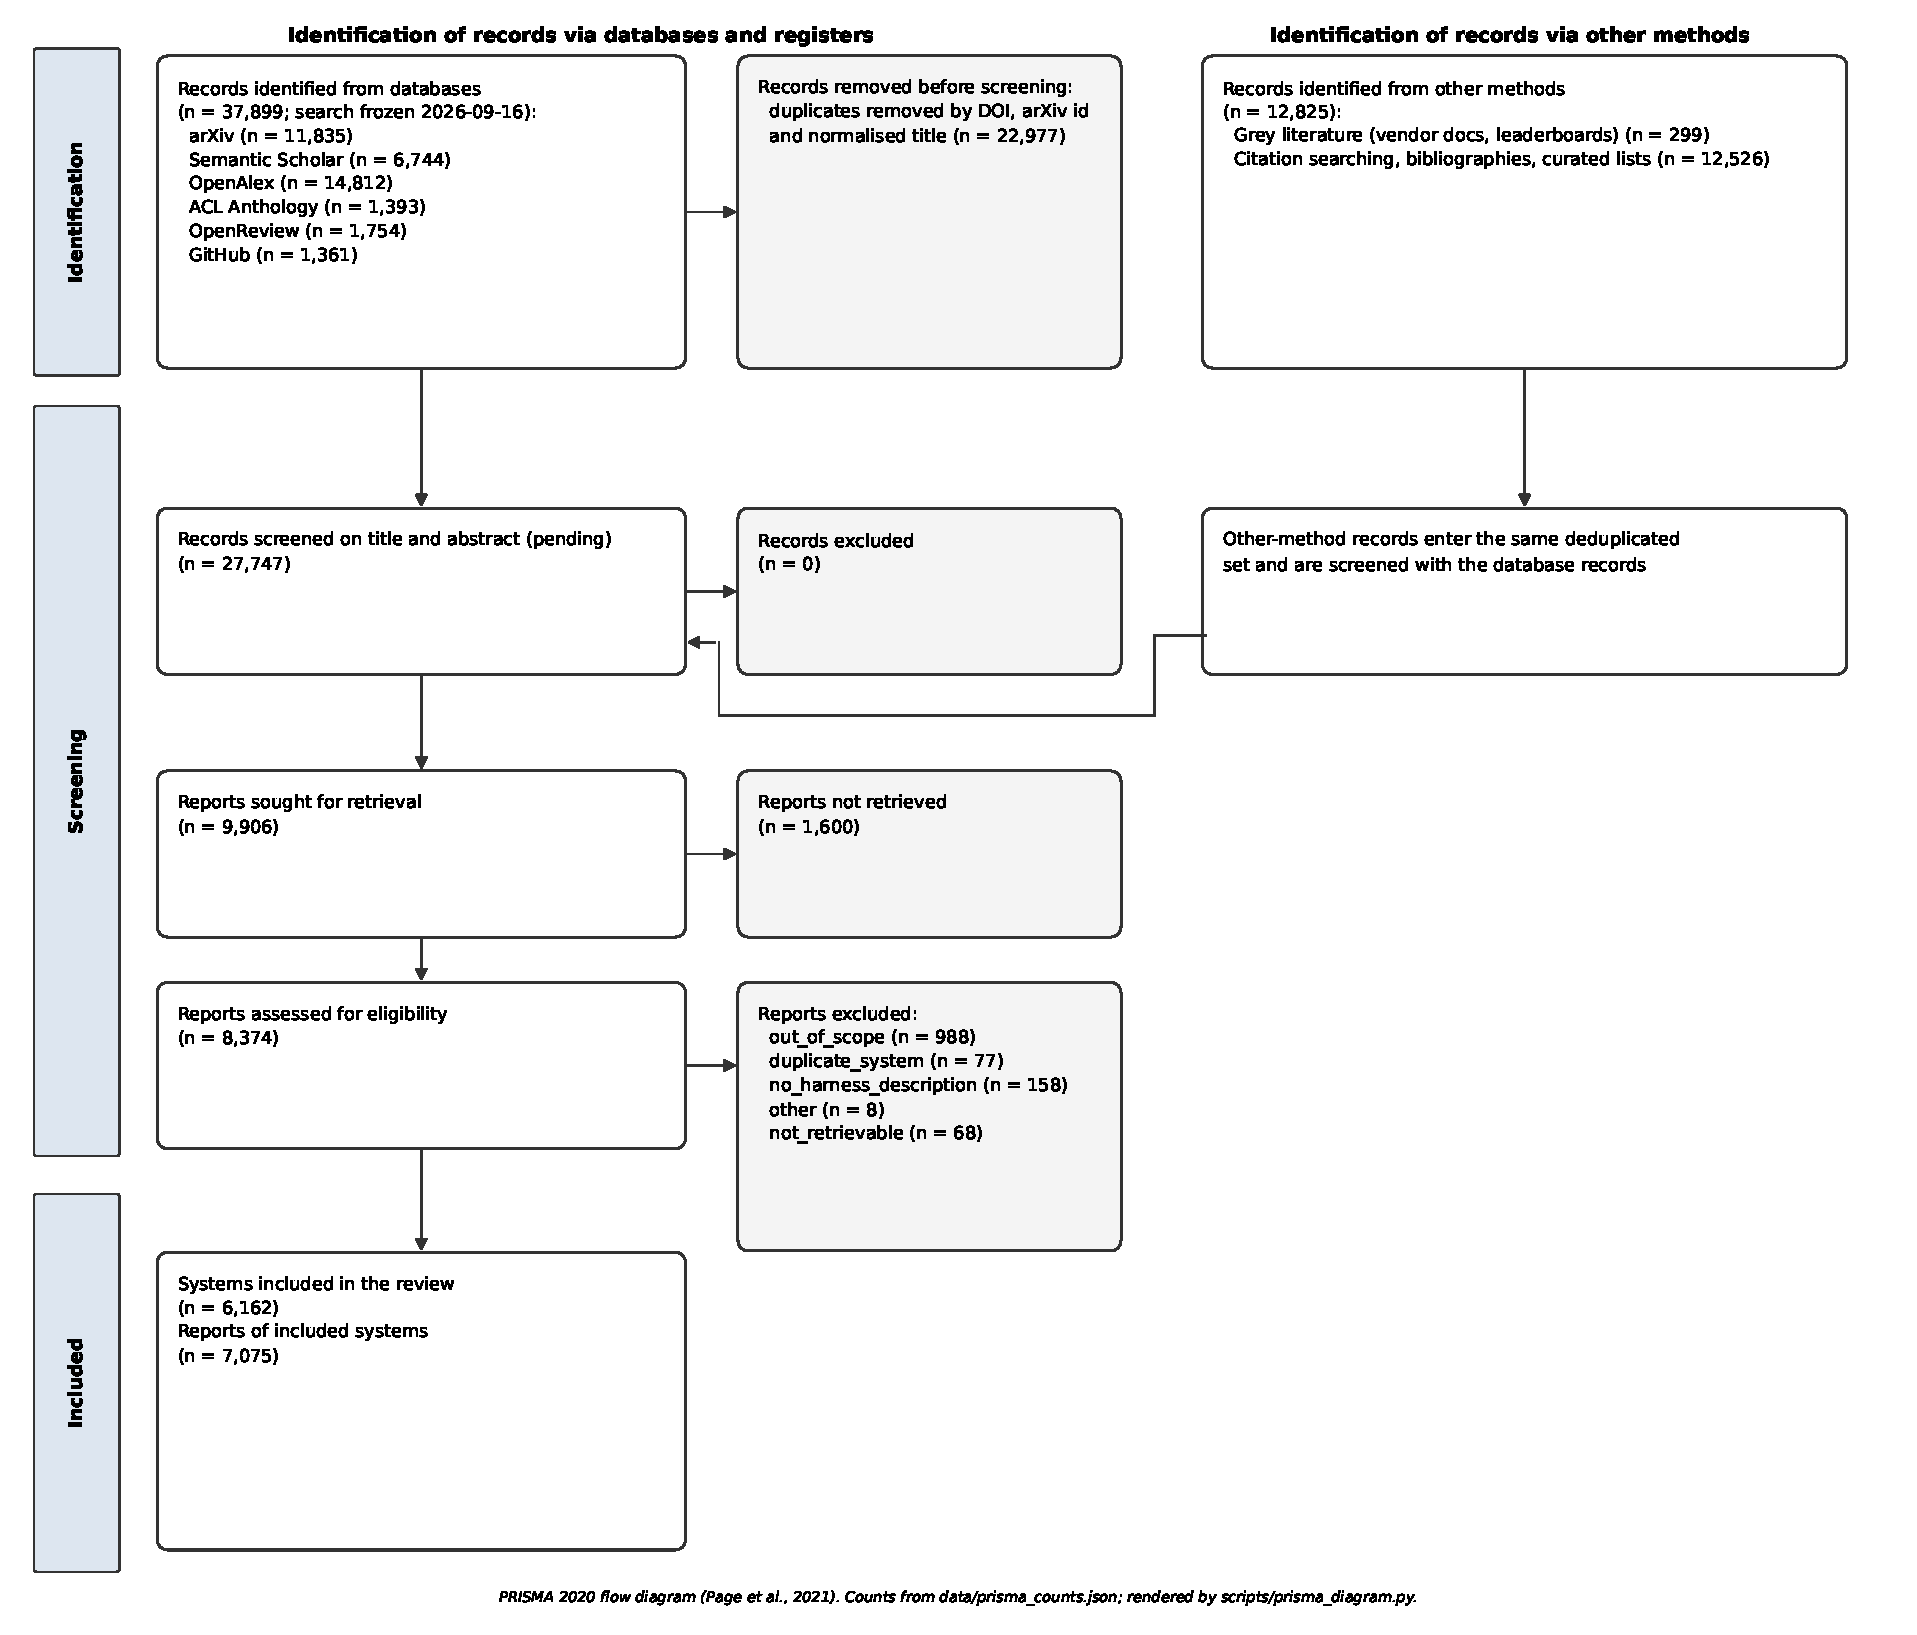
\includegraphics[width=\linewidth]{prisma_flow}
  \caption{PRISMA 2020 flow of records. Left: identification via databases and registers. Right: the
  supplementary independent arm of amendment~7. The ``included systems'' box (6,504) is the sampling frame
  of \S\ref{subsec:grouping}, regenerated after the grouping repair of amendment~10.}
  \label{fig:prisma}
\end{figure}

\subsection{Two-Tier Escalation Screening}\label{subsec:selection}

Two-Tier Escalation Screening (Figure~\ref{fig:screening-framework}) spends second readings where a
first reading is least trustworthy, because a single model reading cannot report its own error. It has
four modules.

\begin{figure}[t]
  \centering
  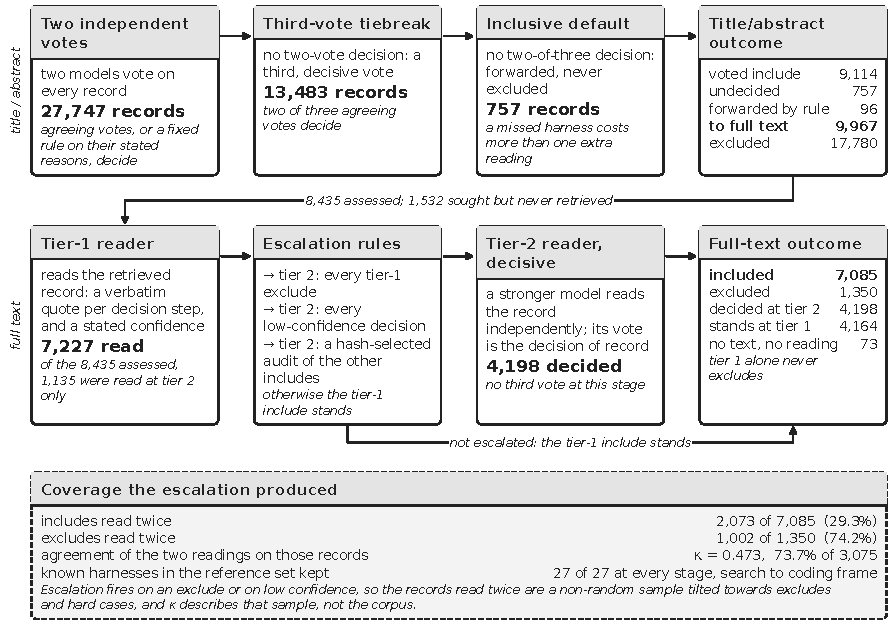
\includegraphics[width=\linewidth]{screening_framework}
  \caption{Two-Tier Escalation Screening. At title and abstract, two independent votes, a rule-based triage
  and a third-vote tiebreak; unsettled records are forwarded. At full text, a tier-1 reading of the
  evidence bundle, an escalation rule that sends exclusions, low-confidence decisions and an audit sample to
  a tier-2 decisive reading.}
  \label{fig:screening-framework}
\end{figure}

\emph{Tier-1 reading.} Given a record, the first reading applies the protocol's decision procedure and
returns a decision, a reason and the deciding step. At title and abstract every candidate receives two
independent first-reading votes, include, exclude or unsure. At full text the reading must
quote the evidence bundle verbatim for every step of the twelve-step procedure it reaches, so each
decision is checkable against its source.

\emph{Escalation rule.} At full text, every tier-1 exclude, every low-confidence tier-1 decision and a
hash-selected 10\% of the remaining tier-1 includes are escalated; records first read at tier~2 receive a
hash-selected 20\% tier-1 reading. Escalating exclusions targets the error a review cannot recover later.

\emph{Tier-2 decisive reading.} The escalation stage re-reads an escalated record independently, and its
decision is the decision of record, so no tier-1 exclusion stands without a second reading.

\emph{Third-vote tiebreak.} At title and abstract, a rule-based triage settles hard-rule cases and records
on which the two votes agree. The 13,483 it cannot settle receive a third vote that sees both priors and
may answer only include or exclude. Records three votes leave unsettled are forwarded, never excluded.

The price of concentrating second readings where errors cost most is uneven coverage:
2,073 of 7,085 includes (29.3\%) and 1,002 of 1,350 excludes (74.2\%) were read twice. On those 3,075
records Cohen's kappa \citep{cohen1960kappa} is 0.473, an estimate for a sample enriched in disputed
scope-boundary records, not for a random record. Two checks in Table~\ref{tab:screening-checks} stand in
for human verification: recall of 27 of 27 on a reference set drawn from our must-cite list and three
prior catalogues \citep{rombaut2026insidescaffold,barbaste2026anatomy,meng2026harnesssurvey}, and the
independent pipeline's agreement of 0.843 (kappa 0.664). Neither estimates accuracy on obscure systems.

\begin{table}[t]
  \footnotesize
  \caption{Checks on Two-Tier Escalation Screening. Agreement figures compare two model readings and measure
  consistency; only the external checks bear on accuracy. Interval: 95\%, Wilson
  \citep{wilson1927interval} for recall.}
  \label{tab:screening-checks}
  \begin{tabular}{@{}l l r r l r@{}}
    \toprule
    Stage & Check & $n$ & Estimate $\uparrow$ & 95\% interval & $\kappa$ $\uparrow$ \\
    \midrule
    Title/abstract & Two-vote agreement, three classes & 27,747 & 0.716 & --- & 0.564 \\
                   & Two-vote agreement, exclude vs.\ forward & 27,747 & 0.821 & --- & 0.616 \\
    \midrule
    Full text & Two-reading agreement & 3,075 & 0.737 & [0.721, 0.752] & 0.473 \\
              & Tier-1 includes confirmed at second reading & 2,073 & 0.677 & --- & --- \\
              & Quotes found verbatim in the text shown & 60,881 & 0.960 & --- & --- \\
    \midrule
    External & Reference-set recall, search to coding frame & 27 & 1.000 & [0.875, 1.000] & --- \\
             & Negative reference set excluded as intended & 13 & 1.000 & --- & --- \\
             & Agreement with an independent pipeline & 434 & 0.843 & --- & 0.664 \\
             & Independent pipeline's includes in our pool & 411 & 0.749 & --- & --- \\
    \bottomrule
  \end{tabular}
\end{table}

\subsection{System grouping}\label{subsec:grouping}

Coding records would count a well-documented harness many times, so includes were grouped into systems
by repository, then by name similarity, then by the registered versioning rule. Amendment~10 repaired two
defects: transitive fuzzy matching, chaining pairs each just above threshold, pooled 129 records carrying
105 distinct names into one row, and normalization collapsed ``Agent S'' and ``Agents'' into one key. A
name similarity now never merges records with different known repositories, and without a repository
the normalized names must be equal. The repaired grouping yields the 6,504-system frame of
Figure~\ref{fig:prisma}, with reference-set recall unchanged at 27 of 27, at the accepted cost of
under-merging: a project spread over several repositories can yield more than one row.

\subsection{Evidence-Anchored Coding}\label{subsec:coding}

Evidence-Anchored Coding (Figure~\ref{fig:coding-framework}) makes every cell re-checkable against the
text it was read from, on the 38 dimensions of schema v1.0.0, which no coding step changed. It has five
modules and a release gate.

\begin{figure}[t]
  \centering
  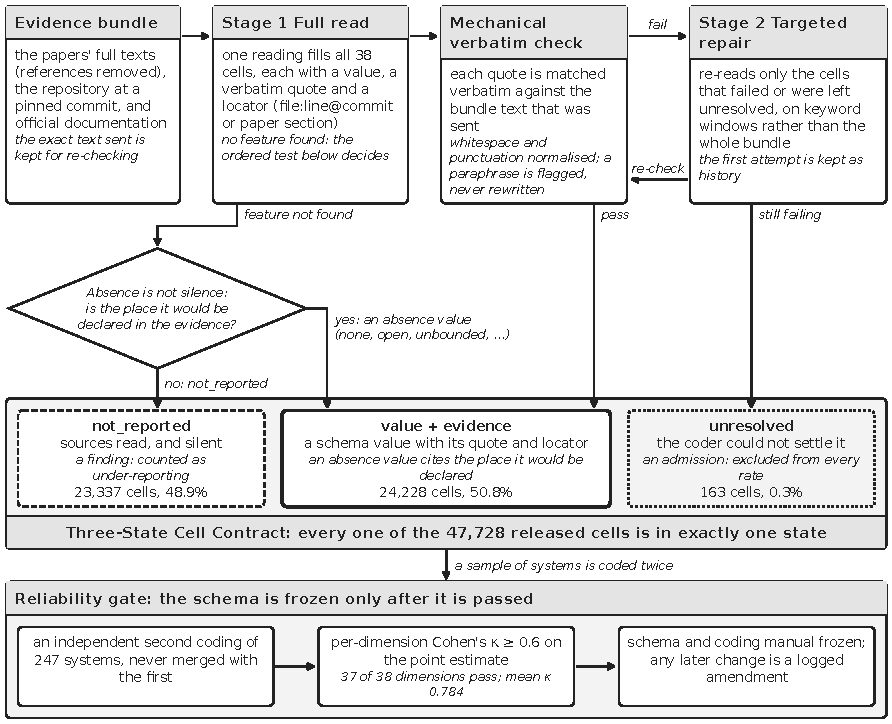
\includegraphics[width=\linewidth]{coding_framework}
  \caption{Evidence-Anchored Coding. An evidence bundle is read in full (Stage~1); every quote is verified
  verbatim against the text shown; unverified or unsettled cells are re-read from targeted windows
  (Stage~2); each cell is assigned one state of the Three-State Cell Contract; systems with at least 19 of
  38 dimensions settled enter the release.}
  \label{fig:coding-framework}
\end{figure}

\emph{Evidence bundle.} Given a system, we first assemble its paper, its repository at the pinned version
and its official documentation, so the bundle holds the configuration surfaces where features are
declared. A paper alone understates what a harness does: in the full-text pilot, paper-only evidence excluded 11 of
15 reference systems (amendment~5).

\emph{Stage~1: full reading.} The coder then reads the whole bundle once and returns all 38 cells, each with
a value, a verbatim quote, a locator, a confidence and the coder identifier. The coding manual's rules are
assembled into the coder's instructions for every system, so an amendment reaches coder and validator
together. Repository locators name file and commit without a line, because the bundle carries no line
numbers and demanding them would invite fabricated ones (amendment~8).

\emph{Verbatim verification.} Every quote is compared character for character, after whitespace and
punctuation normalization, with the exact text the coder was sent. A paraphrase, or a cell that breaks its
dimension's shape or a manual rule, is flagged and never repaired into a plausible value, so no cell's
evidence rests on the coder's say-so.

\emph{Stage~2: targeted repair.} Only cells that Stage~1 left unresolved, invalid or unverified are re-read,
from keyword windows around the dimension's key terms. A settled Stage-2 cell supersedes its Stage-1
attempt, which is kept. This recovers what a long single reading misses without re-coding what is
already verified.

\emph{Three-State Cell Contract.} Finally, the ordered rule of Table~\ref{tab:absence-rule} puts every
cell in one of the three states of \S\ref{subsec:cellstates}. The under-reporting result (RQ4) is a count
of silence: coding silence as absence would turn an undocumented feature into a missing one, and pooling
our failures with silence would inflate the silence rate with our own errors. Of the 47,728 released
cells, 163 (0.3\%) are \texttt{unresolved}, and they are excluded from every under-reporting rate.

\begin{table}[t]
  \footnotesize
  \caption{The ordered ``absence is not silence'' rule of the Three-State Cell Contract. Steps are applied in
  order and the first that holds decides the cell. Prose that does not mention a feature is never evidence
  that it is absent.}
  \label{tab:absence-rule}
  \begin{tabular}{@{}l p{0.40\linewidth} p{0.30\linewidth} l@{}}
    \toprule
    Step & Condition on the evidence bundle & Coded as & State \\
    \midrule
    1 & A verbatim passage states the feature's value & That value, with quote and locator & value \\
    2 & The place where the feature would be declared (config schema, CLI flags, tool registry, run loop,
        documented feature list) is present, and the feature is not in it & The absence value
        (\texttt{none}, \texttt{open}, \ldots), citing that place; confidence at most medium & value \\
    3 & No such place is in the bundle (no config surface, truncated repository, paper only) &
        \texttt{not\_reported}, naming the missing place & \texttt{not\_reported} \\
    4 & The cell cannot be settled, or breaks its dimension's shape or a manual rule &
        Flagged, never repaired & \texttt{unresolved} \\
    \bottomrule
  \end{tabular}
\end{table}

\emph{Release gate.} A system enters the release when at least 19 of its 38 dimensions are settled.
Demanding all 38 would have admitted 77 of the 1,116 systems coded when this was last measured; the
gate buys coverage at the price of partial rows, which the contract marks cell by cell. Of the 1,257
systems coded, 1,256 form the released dataset; the other one's identifier is a reserved device name on
the build platform, so its file cannot be written.

\subsection{Reliability gate}\label{subsec:reliability}

The schema was frozen only after a registered gate: per-dimension Cohen's kappa of at least 0.6. A
deterministic 20\% sample of the coded set was coded a second time, independently, through Stage~1 and
Stage~2, so the comparison measures the whole procedure; the two codings were never merged. The draw
names 245 systems; 247 were double-coded, and reliability is computed on all 247 rather than trimmed to
the draw. In Table~\ref{tab:reliability}, 37 of 38 dimensions clear the floor on the point estimate. A
cluster bootstrap over systems leaves four dimensions whose interval includes 0.6, and only
\texttt{loop\_primitives} sits below it; it is kept and flagged, not redefined
(\S\ref{subsec:multivalued}). Gwet's AC1 \citep{gwet2008ac1} is
reported beside kappa because kappa is depressed when one value dominates
\citep{feinstein1990paradoxes,byrt1993kappa}, as it does wherever \texttt{not\_reported} is modal. No
kappa on the 247 is stacked over all 38 dimensions' cells, because a chance baseline spanning 38 value spaces
inflates it by construction. The 217 systems of the
amendment-9 validation and the 247 here are different samples, not a corrected figure. Both readings are
model readings under the same instructions, so these figures measure reproducibility, not correctness or
agreement with a human coder.

\begin{table}[t]
  \footnotesize
  \caption{Reliability gate. Top: the double-coded sample, with 95\% percentile cluster-bootstrap
  intervals over systems (2,000 draws). Middle: the four dimensions whose kappa interval includes the
  registered floor of 0.6. Bottom: amendment-9 validation on the earlier 217-system sample, Stage~1 only,
  before and after the rewrite. Both readings are model readings: every row measures reproducibility.}
  \label{tab:reliability}
  \begin{tabular}{@{}l r r@{}}
    \toprule
    Quantity & Estimate & 95\% interval \\
    \midrule
    Double-coded systems / cell pairs & 247 / 9,386 & --- \\
    Observed agreement $\uparrow$ & 0.870 & [0.859, 0.881] \\
    Mean per-dimension $\kappa$ $\uparrow$ & 0.784 & [0.765, 0.800] \\
    Mean per-dimension AC1 $\uparrow$ & 0.855 & [0.842, 0.867] \\
    Dimensions with $\kappa \geq 0.6$, point estimate & 37 of 38 & --- \\
    \midrule
    $\kappa$, \texttt{loop\_primitives} & 0.590 & [0.523, 0.657] \\
    $\kappa$, \texttt{edit\_primitive} & 0.628 & [0.537, 0.711] \\
    $\kappa$, \texttt{network\_policy} & 0.668 & [0.527, 0.793] \\
    $\kappa$, \texttt{retry\_policy} & 0.675 & [0.587, 0.765] \\
    \midrule
    Amendment 9, pooled agreement (before $\to$ after) & 0.597 $\to$ 0.872 & --- \\
    Amendment 9, stacked $\kappa$ (before $\to$ after) & 0.564 $\to$ 0.832 & --- \\
    Amendment 9, stacked AC1 (before $\to$ after) & 0.596 $\to$ 0.872 & --- \\
    Amendment 9, \texttt{not\_reported} share of cells (before $\to$ after) & 0.269 $\to$ 0.483 & --- \\
    \bottomrule
  \end{tabular}
\end{table}

\paragraph{Outcome data.} Collected in the same reading as the design cells, every reported benchmark
score is released with its benchmark, split, metric, base model and the passage it was read from, and
no score enters without that passage.
Within-study ablation contrasts are classified from the same extraction, and every dropped candidate row
is published with its reason, so the recall of the harvest in Section~\ref{sec:outcomes} can be audited.

\subsection{Synthesis}\label{subsec:synthesis}

The coded set is a stratified sample of the 6,504-system frame, drawn with a fixed seed (amendment~6;
definitions in Supplement~S4): a census of stratum H, the visible systems (984, weight 1); 150 of the 683
peer-reviewed systems with code in P (weight 4.5533); and 100 of the 4,837 others in O (weight 48.37).
Field-level claims are weighted, with design standard errors taking the system as the sampling unit,
over the 1,233 released systems of the
1,234 drawn, because the weights are the draw's inverse inclusion probabilities. The other 23 released
systems, several of them benchmark reference agents the recall check required, were coded outside the
draw and carry weight 0. Coded-set claims are unweighted over all 1,256, and every proportion says which
it is.

Supplement~S6 tabulates the estimator behind each synthesis question with the test that could
overturn it: weighted proportions with design standard errors, or unweighted ones with Wilson
intervals; Miller--Madow entropy; bias-corrected Cram\'er's V; Gower-distance clustering;
within-key standardized contrasts with permutation tests; random-effects pooling of ablations with
$I^2$ \citep{higgins2002heterogeneity} and prediction intervals; and sign, own-arm and funnel tests of
reporting bias, with Benjamini--Hochberg control within each test family. Two choices need a reason.
Diversity over time is unweighted, one system one vote, because a weighted entropy would rest on a
handful of stratum-O systems per dimension-year cell. Design families had to pass the three bars of
Table~\ref{tab:landscape_bars}, stated before clustering, with stability measured over 200 subsamples at
80\% and a silhouette null that preserves each dimension's marginals and missingness and passes through
the same eligibility filter and maximization over $k$ as the data. A partition failing any bar is
reported as evidence against families.

\paragraph{Reporting bias and certainty.}\label{subsec:reportingbias}
Risk of bias in the sources is assessed against five cross-cutting caveats: benchmark versioning,
contamination, self-reporting, harness--model entanglement and scaffold drift. No GRADE-style rating is
applied, because the outcome evidence is author-reported scores on heterogeneous benchmarks rather than
comparative trials. Certainty is reported per estimate instead, as a bound direction, a discount, a
prediction interval beside the confidence interval, and, for every null, the minimum detectable effect.
The registered mixed-effects regression was not fitted because the comparable data cannot identify it
(amendment~11).

\subsection{Implementation and disclosure}\label{subsec:llmdisclosure}

Model instances applying the registered protocol made every screening, coding and label-classification
decision (Table~\ref{tab:implementation}), and no human verified any coded cell or screening decision
(amendment~4). The author wrote the protocol, definition, coding manual, schema and every analysis, made
every amendment decision, and is responsible for the claims; the models supplied the readings. Coding
ran with tools disabled, one system per call, and schema validation on every cell. Two
offensive-security systems, \texttt{cai} and \texttt{pentagi}, halted the primary model's safety
classifier mid-response on repeated attempts and were read by Claude Sonnet 5, which leaves more cells
unresolved on identical bundles; the first stage of fifteen further systems, most of them security
agents, was read by Claude Opus 5 (Table~\ref{tab:implementation}); every row records its model. At screening, batches containing such
systems were re-read one document per call, which cleared every refusal. Mechanical checks replace human
verification: verbatim quote matching, schema validation, a public per-record audit page, reference-set
recall, second readings and the independent cross-check.

\begin{table}[t]
  \footnotesize
  \caption{Models and instruction versions by stage. Volume is records unless the row names its unit;
  full-text rows count decisions of record. Every decision listed was made by a model; none was verified
  by a human.}
  \label{tab:implementation}
  \begin{tabular}{@{}p{0.25\linewidth} p{0.33\linewidth} l r@{}}
    \toprule
    Stage & Model & Instruction version & Volume \\
    \midrule
    Title/abstract, first vote & Claude Opus 5 & \texttt{ta-v1-2026-09-17} & 21,480 \\
     & Claude Sonnet 5 & \texttt{ta-v1-2026-09-17} & 6,267 \\
    Title/abstract, second vote & The other model & \texttt{ta-v1-2026-09-17} & 27,747 \\
    Title/abstract, third vote & Claude Opus 5, Claude Sonnet 5 & \texttt{ta-v2-tiebreak-2026-09-17} &
      13,483 \\
    \midrule
    Full text, tier 1 & Claude Sonnet 5 & \texttt{ft-v2-2026-09-18} & 4,164 \\
    Full text, tier 2 & Claude Opus 5 (4,126); Claude Opus 4.8, seven batches (56); Claude Sonnet 5 (16)
      & \texttt{ft-v2-2026-09-18} & 4,198 \\
    Full text, not retrievable & No model call & --- & 73 \\
    \midrule
    Coding, Stages 1 and 2 & Claude Opus 5.5 (Stage~1 of 15 systems: Claude Opus 5; of two: Claude
      Sonnet 5) & \texttt{code-v2-2026-09-23} & 1,257 systems \\
    Ablation labels, coded set & Claude Opus 5.5, confidence floor 0.5 & --- & 1,008 labels \\
    Ablation rows, corpus-wide & Claude Sonnet 5 & \texttt{corpus-ablation-v1-2026-09-25} &
      \rqCorpusPapersExtracted{} papers \\
    Comparator aliases & Claude Opus 5.5 & \texttt{alias-v1-2026-09-24} & 555 pairs \\
    Controlled-ablation pilots & Claude Sonnet 5, Claude Haiku 4.5 (generators) & \texttt{tier3-v1},
      \texttt{tier3-v2-12a} & 654 runs \\
    \bottomrule
  \end{tabular}
\end{table}

\section{The unified taxonomy}\label{sec:taxonomy}

Harness design decomposes into 38 separately coded choices in nine layers, not into a small number of
architectures. Figure~\ref{fig:taxonomy-map} draws the structure and Table~\ref{tab:dimensions} lists
every dimension with the size of its value set. Each dimension is a question a reader can put to any
system, answer from a pinned artifact, and support with a cited line. The coded corpus fits this premise
better than a family structure: clustering falls short of both pre-stated floors for silhouette and
bootstrap stability (verdict negative), and on pairs where both dimensions carry a value the mean
corrected Cram\'er's $V$ is 0.167 across 666 pairs (\S\ref{sec:landscape}), which is what a space of
loosely related choices looks like when it is measured.

\begin{figure}[t]
\centering
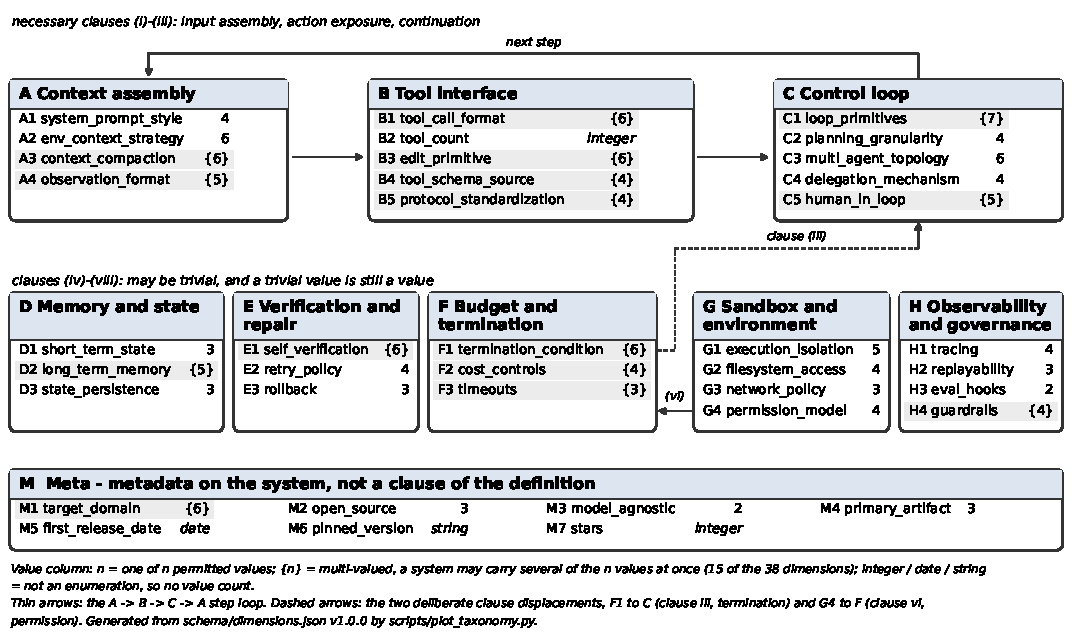
\includegraphics[width=\linewidth]{taxonomy_map}
\caption{The unified taxonomy, generated from the frozen schema so it cannot drift from it. Top row: the
three necessary clauses, whose composition is the step loop
$\mathbf{A}\rightarrow\mathbf{B}\rightarrow\mathbf{C}\rightarrow\mathbf{A}$. Second row:
clauses~(iv)--(viii), which may be trivial; a trivial value is still a value, never
\texttt{not\_reported}. \textbf{M} carries metadata, not a clause. Dashed arrows: the deliberate
displacements of \textbf{F1} (clause~(iii)) and \textbf{G4} (clause~(vi)). Value counts as in
Table~\ref{tab:dimensions}.}
\label{fig:taxonomy-map}
\end{figure}

% Generated from the frozen schema by the Section 5 table generator; do not edit by hand.
% One float: main.tex does not load longtable, and the 38 single-line rows fit one float.
\begin{table}[tbp]
\caption{The 38 dimensions of the frozen schema (v1.0.0), grouped by layer. \emph{Values}: $n$ is
the size of a single-valued enumeration; $\{n\}$ is the size of a multi-valued one, whose cell holds a
set; a type name marks the four dimensions that are not enumerations. Full value sets, the judgment
call for each layer, and two worked examples are in Supplement~S1.}
\label{tab:dimensions}
\footnotesize
\begin{tabular}{@{}l l l l r@{}}
\toprule
Layer & ID & Key & What it records & Values \\
\midrule
A\enspace Context & A1 & \texttt{system\_prompt\_style} & how the per-call system prompt is produced & 4 \\
\phantom{A}\enspace assembly & A2 & \texttt{env\_context\_strategy} & how the model learns the repository or environment & 6 \\
 & A3 & \texttt{context\_compaction} & mechanisms that shrink the history sent & $\{6\}$ \\
 & A4 & \texttt{observation\_format} & format in which tool results reach the model & $\{5\}$ \\
\midrule
B\enspace Tool interface & B1 & \texttt{tool\_call\_format} & syntax by which the model requests actions & $\{6\}$ \\
 & B2 & \texttt{tool\_count} & tool definitions exposed at the default configuration & \emph{integer} \\
 & B3 & \texttt{edit\_primitive} & how the model expresses a file edit & $\{6\}$ \\
 & B4 & \texttt{tool\_schema\_source} & where the tool schema comes from & $\{4\}$ \\
 & B5 & \texttt{protocol\_standardization} & standard agent or tool protocols spoken & $\{4\}$ \\
\midrule
C\enspace Control loop & C1 & \texttt{loop\_primitives} & control-flow patterns driving calls and actions & $\{7\}$ \\
 & C2 & \texttt{planning\_granularity} & whether and how a plan is represented & 4 \\
 & C3 & \texttt{multi\_agent\_topology} & arrangement of agents at the default & 6 \\
 & C4 & \texttt{delegation\_mechanism} & how work is handed to another agent & 4 \\
 & C5 & \texttt{human\_in\_loop} & points where a human gates or steers & $\{5\}$ \\
\midrule
D\enspace Memory and & D1 & \texttt{short\_term\_state} & working state kept within a run & 3 \\
\phantom{D}\enspace state & D2 & \texttt{long\_term\_memory} & information persisted across runs and re-injected & $\{5\}$ \\
 & D3 & \texttt{state\_persistence} & whether an interrupted run can continue & 3 \\
\midrule
E\enspace Verification & E1 & \texttt{self\_verification} & checks the harness applies to the work & $\{6\}$ \\
\phantom{E}\enspace and repair & E2 & \texttt{retry\_policy} & task-level retry after a failed attempt & 4 \\
 & E3 & \texttt{rollback} & mechanism that reverts changes made in the run & 3 \\
\midrule
F\enspace Budget and & F1 & \texttt{termination\_condition} & conditions that end a run & $\{6\}$ \\
\phantom{F}\enspace termination & F2 & \texttt{cost\_controls} & mechanisms that limit or reduce spend & $\{4\}$ \\
 & F3 & \texttt{timeouts} & time limits the harness enforces & $\{3\}$ \\
\midrule
G\enspace Sandbox and & G1 & \texttt{execution\_isolation} & boundary within which actions execute & 5 \\
\phantom{G}\enspace environment & G2 & \texttt{filesystem\_access} & what the agent may touch inside G1 & 4 \\
 & G3 & \texttt{network\_policy} & network egress available to actions & 3 \\
 & G4 & \texttt{permission\_model} & how individual actions are authorized & 4 \\
\midrule
H\enspace Observability & H1 & \texttt{tracing} & richest run record the harness can emit & 4 \\
\phantom{H}\enspace and governance & H2 & \texttt{replayability} & whether a recorded trajectory can be re-run & 3 \\
 & H3 & \texttt{eval\_hooks} & benchmark evaluation wired into its own repositories & 2 \\
 & H4 & \texttt{guardrails} & safety controls on inputs, outputs, and actions & $\{4\}$ \\
\midrule
M\enspace Meta & M1 & \texttt{target\_domain} & task domains the harness is built for & $\{6\}$ \\
 & M2 & \texttt{open\_source} & whether the source is open & 3 \\
 & M3 & \texttt{model\_agnostic} & whether it runs across model providers & 2 \\
 & M4 & \texttt{primary\_artifact} & artifact the pinned version is coded from & 3 \\
 & M5 & \texttt{first\_release\_date} & first tagged release of the coded line & \emph{date} \\
 & M6 & \texttt{pinned\_version} & tag and commit per coded repository & \emph{string} \\
 & M7 & \texttt{stars} & flagship-repository stars, date-stamped in evidence & \emph{integer} \\
\bottomrule
\end{tabular}
\end{table}

Table~\ref{tab:dimensions} shows an instrument built mostly from small closed lists. Nineteen dimensions
are single-valued enumerations, fifteen hold a set, and four are an integer, a date, or a string; the
enumerations range from two to seven values. Every cell is therefore checkable against a closed list or a
stated counting, dating, or pinning rule, and the table is generated from the schema so that it cannot
drift from what was coded.

A layer is the set of dimensions that answers one clause of the working definition, and layers A to H
follow the clauses in order (\S\ref{subsec:layers}). Two placements depart from that map on purpose. The
termination condition sits in F so that termination policy and budget are reported together, and the
permission model sits in G because in practice it is configured alongside isolation. The ninth layer, M,
is metadata that stratification, weighting, and the time series need. Within a layer, one dimension records one
decision, made at one identifiable place in the pinned artifact, whose value a second reader can
recover from the same evidence. Per-dimension reliability is the test of that criterion: a dimension
that bundles two decisions yields readings that agree on the evidence and disagree on the value.

That criterion is why our cuts differ from prior taxonomies. Guo et al.\ place stopping criteria under
the control loop and budget control under verification and governance~\citep{guo2026qa2task}; a coder
cannot apply that split reliably, so we separate C from F, and E from G4 and H4. Li et al.'s context
layer covers both what the model sees this step and what persists between runs, which we split into A
and D~\citep{li2026harnessengineering}. Nine of Rombaut's twelve source-code dimensions map onto ours,
and that work supplied our evidence standard of a pinned commit with a file and
line~\citep{rombaut2026insidescaffold}. The other three have no dimension of ours to map to;
\S\ref{sec:related} names them and \S\ref{sec:threats} weighs what their omission costs.

\subsection{Multi-valued dimensions}\label{subsec:multivalued}

Fifteen dimensions hold a set, because on them a harness does several things at once: it stacks
compaction mechanisms, ships several call parsers, or gates a run at more than one point. A set cell
records every value reachable through shipped configuration, with the default named in the note. Where a value set contains \texttt{none}, it is a singleton by rule and never appears
beside another value. The registered reliability measure, exact-set agreement, is harsh on these cells:
two readings that agree on all but one primitive score as a complete disagreement, so the penalty grows
with the size of the true set rather than the size of the error. Loop primitives (C1) bears the cost. It
is the one dimension below the 0.6 freeze threshold on exact-set Cohen's kappa (0.590), and it clears
the threshold per value (0.731); Supplement~S1 reports all four measures, each of them
reproducibility between two model readings rather than correctness. We keep C1 and flag it as the
weakest dimension rather than redefine it, because redefining a dimension after seeing its reliability
is the post-hoc repair this paper audits others for.

\subsection{The absence rule}\label{subsec:absence}

The taxonomy separates a design decision from a documentation gap, and the absence rule enforces the
separation. An absence value, such as \texttt{none} or \texttt{open} for network policy, is a value on a
dimension: a choice the builders made. \texttt{not\_reported} is a property of the documents: the
sources were read and are silent. The rule (Table~\ref{tab:absence-rule}) codes an absence value only
when the evidence contains an enumerated place where the feature would be declared, and the feature is
not there; prose that never mentions a feature is never evidence that it is absent. A taxonomy that let
silence imply \texttt{none} would measure documentation while claiming to measure design, and every
distribution over its values would mix the two with no way to separate them. The rule is what lets the
under-reporting result speak about the literature rather than the systems; its history as a protocol
amendment and its measured effect on reliability are in \S\ref{sec:methods}.

\subsection{Boundary cases and known ambiguities}\label{subsec:ambiguities}

Coding two systems end to end, SWE-agent v1.1.0~\citep{yang2024sweagent} and OpenHands
v1.16.0~\citep{wang2024openhands}, raised 26 ambiguities, and each was resolved by a rule in the
coding manual rather than by changing a value set; Supplement~S1 lists all 26 with their resolutions.
Ten follow one of two patterns: code the shipped default and note the reachable alternatives (entries 1
and 13), or record the closest value and write the mismatch in the note (entries 3, 5, 6, 10, 12, 16, 24,
and 25). Entry 17 is the one departure from default-first coding: tracing is coded at the highest level
the artifact can reach, and the note says what runs by default. Table~\ref{tab:ambiguities} gives six.
Publishing the list is part of the instrument, because a reader who disagrees with a resolution can
recode that dimension from the released evidence strings.

% Six of the 26 manual entries; the full list is in the coding-manual supplement (S1).
\begin{table}[tbp]
\caption{Six of the 26 ambiguities recorded while coding the two worked systems, numbered as in the
manual: the two general rules (1, 26), the one departure from default-first coding (17), and three that
settle checklist dimensions (\S\ref{subsec:checklist}). All 26 are in Supplement~S1.}
\label{tab:ambiguities}
\footnotesize
\begin{tabular}{@{}r p{0.17\linewidth} p{0.31\linewidth} p{0.40\linewidth}@{}}
\toprule
\# & Dimension & Ambiguity & Resolution \tabularnewline
\midrule
1 & B2, C3--C5, D3, E1, E2, G1, G4 & \raggedright Capability shipped but off by default & \raggedright Code the default; name reachable alternatives in the note \tabularnewline
2 & B2 & \raggedright Toolsets, built-in, injected, and MCP tools & \raggedright One per schema sent; toolsets expanded; injected tools excluded \tabularnewline
10 & E3 & \raggedright Per-file tool-level undo & \raggedright \texttt{snapshot}; a repository reset is \texttt{git\_based} \tabularnewline
15 & G3 & \raggedright No network configuration anywhere & \raggedright \texttt{open} at medium confidence, citing the configuration surface \tabularnewline
17 & H1 & \raggedright Optional trace exporter versus always-on log & \raggedright Highest available level; default noted \tabularnewline
26 & General & \raggedright Evidence for an absence value & \raggedright The absence rule (\S\ref{subsec:absence}) \tabularnewline
\bottomrule
\end{tabular}
\end{table}

\subsection{Schema freeze}\label{subsec:freeze}

The schema is frozen at v1.0.0 with all 38 dimensions intact: none was added, removed, renamed, or
re-valued between the initial draft and the freeze on 2026-09-23. The freeze was gated on
per-dimension reliability rather than on a date, and the gate, Cohen's kappa of at least 0.6, was met on
37 of 38 dimensions. The one change to the cell contract came before the freeze and added
\texttt{unresolved} beside \texttt{not\_reported}, so that a cell the coder could not settle is never
pooled with a source that is silent. The released schema changelog records every change since the draft, and any
later change needs a changelog line and a registration update, so that the released dataset and this
section describe one instrument. Supplement~S1 carries the per-layer value sets, judgment calls,
decision rules, and worked examples.

\section{The landscape of harness design}
\label{sec:landscape}

Five descriptive findings follow. All five rest on 1,256 systems coded on 38 dimensions, 47,728 cells, weighted to a 6,504-system
frame (Section~\ref{sec:methods}). Field claims use weighted estimates with stratified design standard
errors; claims about what was coded, including clustering and association, are unweighted.

\subsection{The coded set is not the field}
\label{subsec:weighting}

Weighting inverts the modal release artifact: whether a system's canonical release
(\texttt{primary\_artifact}) is a repository, a paper, or a technical report. In the coded set, 867 of
1,252 systems (69.2\%) are repository-primary. Weighted to the frame, repository-primary falls to 33.3\%
and paper-primary rises to 66.0\% $\pm$ 3.0. The mechanism is the stratum design: repository-primary
systems are 746 of 979 in stratum H (76.2\%), which admits systems partly by repository stars, 93 of 157
in P (59.2\%), and 28 of 116 in O (24.1\%). Table~\ref{tab:landscape_flips} places this among seven
dimensions whose modal value changes under weighting. Supplement~S6 shows every value of every
dimension; the distortion is largest for \texttt{primary\_artifact}.

\begin{table}[tbp]
\caption{Dimensions whose modal value changes when the coded set ($n$ reporting systems, unweighted) is
weighted to the frame (estimate $\pm$ one design standard error). Last column: field share of the
coded-set mode, over one standard error below the new mode in the upper block, within one (a tie) in the
lower. Multi-valued shares need not sum to 100\%.}
\label{tab:landscape_flips}
\footnotesize
\begin{tabular}{lrlrlrr}
\toprule
 & & \multicolumn{2}{c}{Coded set} & \multicolumn{2}{c}{Field} & Old mode, \\
\cmidrule(lr){3-4}\cmidrule(lr){5-6}
Dimension & $n$ & Mode & \% & Mode & \% $\pm$ SE & field \% \\
\midrule
\texttt{primary\_artifact}     & 1252 & \texttt{repo}                      & 69.2 & \texttt{paper}           & 66.0 $\pm$ 3.0 & 33.3 \\
\texttt{delegation\_mechanism} &  852 & \texttt{none}                      & 34.2 & \texttt{role\_handoff}   & 50.4 $\pm$ 4.5 & 22.2 \\
\texttt{system\_prompt\_style} &  785 & \texttt{dynamically\_composed}     & 46.1 & \texttt{templated}       & 49.3 $\pm$ 4.5 & 32.8 \\
\texttt{retry\_policy}         &  436 & \texttt{none}                      & 43.6 & \texttt{fixed\_n}        & 45.5 $\pm$ 5.6 & 29.0 \\
\midrule
\texttt{tool\_call\_format}    &  609 & \texttt{native\_function\_calling} & 47.8 & \texttt{json\_in\_text}  & 35.8 $\pm$ 5.4 & 32.2 \\
\texttt{self\_verification}    &  644 & \texttt{llm\_judge}                & 49.2 & \texttt{test\_execution} & 42.1 $\pm$ 4.7 & 40.5 \\
\texttt{permission\_model}     &  385 & \texttt{static\_allowlist}         & 32.7 & \texttt{none}            & 32.0 $\pm$ 9.4 & 28.9 \\
\bottomrule
\end{tabular}
\end{table}

Neither silence nor sampling noise explains the inversion away. \texttt{primary\_artifact} is the
best-documented dimension, with three \texttt{not\_reported} cells, one \texttt{unresolved}, and a
weighted \texttt{not\_reported} rate of 0.05\%, and a design standard error of 3.0 points cannot span
69.2\% to 33.3\%. The same test sorts the other six flips: three are clear reversals, and three are ties
within one standard error. The \texttt{stars} popularity bin also changes mode, but it measures
visibility rather than design and is not counted.

The price of the design is precision where the weights are largest: one coded system in stratum O
stands for 48.37 in the frame. Of the 487 systems that document protocol standardization, 400 name MCP
(82.1\%), but the weighted estimate of 68.4\% carries a design standard error of 12.2 points, too wide
to support a claim about MCP adoption in either direction. The weighting corrects for sampling within
the frame, not for systems the search missed.

Prior harness surveys characterize the systems visible enough to study
\citep{li2026harnessengineering,meng2026harnesssurvey,guo2026qa2task,rombaut2026insidescaffold,barbaste2026anatomy,zhong2026responsibilities,harnesscategorical2026}.
That choice suits a source-code study of eleven systems \citep{barbaste2026anatomy}. Carried over to a
claim about the field, it changes the modal value of seven of 38 dimensions, one of which is the
release artifact itself.

\subsection{Systems document what they do, not how they are bounded}
\label{subsec:underreporting}

Silence concentrates in the layers that bound a harness, not in the layers that drive it
(Table~\ref{tab:landscape_layers}). The weighted rate climbs from 24.9\% $\pm$ 1.2 for the control loop
to 81.6\% $\pm$ 1.8 for sandbox and environment; with standard errors of at most 2.3 points, the
ordering of the extremes is not a sampling accident. All five of the least-documented dimensions
describe what an operator needs to know before deploying an agent.

\begin{table}[tbp]
\caption{Share of cells whose sources are silent (\texttt{not\_reported}), by layer (ordered by field
rate) and for the five least-documented dimensions. The base excludes \texttt{unresolved} cells and
counts cells for a layer, systems for a dimension. Coded set: unweighted; field: weighted estimate $\pm$
one design standard error.}
\label{tab:landscape_layers}
\footnotesize
\begin{tabular}{llrrrr}
\toprule
 & & Dims & Base & Coded set (\%) & Field (\% $\pm$ SE) \\
\midrule
C & Control loop                 & 5 & 6250 & 27.1 & 24.9 $\pm$ 1.2 \\
M & Meta                         & 7 & 8782 & 27.4 & 34.6 $\pm$ 1.3 \\
A & Context assembly             & 4 & 5005 & 44.4 & 40.2 $\pm$ 2.0 \\
E & Verification and repair      & 3 & 3761 & 65.0 & 60.9 $\pm$ 2.3 \\
D & Memory and state             & 3 & 3751 & 52.7 & 63.3 $\pm$ 2.1 \\
F & Budget and termination       & 3 & 3758 & 61.5 & 65.1 $\pm$ 2.0 \\
B & Tool interface               & 5 & 6234 & 63.4 & 71.4 $\pm$ 2.0 \\
H & Observability and governance & 4 & 5014 & 59.7 & 72.8 $\pm$ 2.0 \\
G & Sandbox and environment      & 4 & 5010 & 66.6 & 81.6 $\pm$ 1.8 \\
\midrule
G & \texttt{network\_policy}     & 1 & 1253 & 84.8 & 93.3 $\pm$ 1.5 \\
H & \texttt{replayability}       & 1 & 1256 & 85.1 & 90.6 $\pm$ 2.0 \\
G & \texttt{filesystem\_access}  & 1 & 1254 & 71.0 & 87.5 $\pm$ 2.0 \\
E & \texttt{rollback}            & 1 & 1254 & 81.1 & 86.4 $\pm$ 2.4 \\
D & \texttt{state\_persistence}  & 1 & 1254 & 68.9 & 86.2 $\pm$ 2.1 \\
\bottomrule
\end{tabular}
\end{table}

Weighting sharpens the asymmetry rather than creating it: the field is more silent than the coded set
on layers B, D, F, G, H, and M, and less on A, C, and E. Per dimension (all 38 in Supplement~S6), it
raises silence most for \texttt{open\_source}, \texttt{protocol\_standardization}, and
\texttt{execution\_isolation}, and lowers it for most control-loop dimensions; \texttt{open\_source}
goes from 478 of 1,254 coded systems (38.1\%) to a weighted 69.7\% $\pm$ 3.0. A review that codes only
visible systems understates the silence on what bounds an agent. Every one of these rates measures documents:
\texttt{not\_reported} means the admitted sources were read and are silent, not that a system has no network policy,
no sandbox, or no rollback; a harness may isolate execution well and never say so.

The diagnostic that could have reversed this result nearly did. Before amendment~9
(Section~\ref{sec:methods}), a search that found nothing was an absence value under one rule and
\texttt{not\_reported} under another, an ambiguity behind 19 of the dimensions that failed the
reliability threshold. On the 217-system validation sample the rewrite moved the \texttt{not\_reported}
share from 26.9\% to 48.3\%; the corrected corpus-wide rate is 48.9\% of all 47,728 cells. The
pre-amendment figure was the flattering one, reading prose that never mentioned rollback as evidence that
rollback was absent; the superseded coding is released so the change can be audited.

Two caveats survive. A sandbox documented only in a source the protocol does not admit, such as a blog
post, counts as silent. A layer's rate averages three to seven dimensions, so specific claims should rest
on dimension rows. The published record describes what a harness does far better than what bounds it,
and any secondary analysis of this literature inherits that asymmetry.

\subsection{Coded-set design diversity rose on six dimensions and fell on three}
\label{subsec:convergence}

In the coded set, diversity rose on six dimensions, fell on three, and was stable on 25. For the 34 dimensions with two or more usable
years, we compared the Miller--Madow corrected Shannon entropy \citep{paninski2003entropy} of the first
and last usable year, bootstrapping the change and suppressing cells under 20 reporting systems. Ten
intervals exclude zero, against 1.7 expected under the global null. Nine survive a Benjamini--Hochberg
correction across the 34 tests at $q < 0.05$: six diversifications and three convergences
(Table~\ref{tab:landscape_entropy}), all unweighted coded-set estimates, not estimates for the field.

\begin{table}[tbp]
\caption{The 10 of 34 tested dimensions whose bootstrap interval on the entropy change excludes zero.
$\Delta H$: change in Miller--Madow corrected entropy (nats), first to last usable year. $q$:
Benjamini--Hochberg adjusted bootstrap $p$ across the 34 tests. \texttt{loop\_primitives}' lower bound
has four decimals because it rounds to zero at two. Unweighted coded-set estimates.}
\label{tab:landscape_entropy}
\footnotesize
\begin{tabular}{llrlrl}
\toprule
Dimension & Years & $\Delta H$ (nats) & 95\% CI & $q$ $\downarrow$ & Survives BH \\
\midrule
\multicolumn{6}{l}{\emph{Falls (convergence)}} \\
\texttt{env\_context\_strategy}   & 2023--2026 & $-0.52$ & [$-0.64$, $-0.27$]  & 0.023 & yes \\
\texttt{short\_term\_state}       & 2023--2026 & $-0.27$ & [$-0.42$, $-0.06$]  & 0.029 & yes \\
\texttt{state\_persistence}       & 2024--2026 & $-0.27$ & [$-0.40$, $-0.10$]  & 0.027 & yes \\
\midrule
\multicolumn{6}{l}{\emph{Rises (diversification)}} \\
\texttt{termination\_condition}   & 2023--2026 & $+0.76$ & [$+0.48$, $+1.21$]  & 0.023 & yes \\
\texttt{human\_in\_loop}          & 2024--2026 & $+0.69$ & [$+0.45$, $+1.03$]  & 0.023 & yes \\
\texttt{edit\_primitive}          & 2023--2026 & $+0.60$ & [$+0.18$, $+1.22$]  & 0.027 & yes \\
\texttt{tool\_schema\_source}     & 2023--2026 & $+0.42$ & [$+0.10$, $+0.86$]  & 0.029 & yes \\
\texttt{cost\_controls}           & 2024--2026 & $+0.27$ & [$+0.09$, $+0.52$]  & 0.045 & yes \\
\texttt{rollback}                 & 2024--2026 & $+0.20$ & [$+0.04$, $+0.46$]  & 0.042 & yes \\
\texttt{loop\_primitives}         & 2023--2026 & $+0.14$ & [$+0.0012$, $+0.66$] & 0.177 & no \\
\bottomrule
\end{tabular}
\end{table}

The fastest diversifiers govern when a harness stops and who may interrupt it.
\texttt{termination\_condition} gains the most entropy, its observed value count rising from 9 to 32,
followed by \texttt{human\_in\_loop} and \texttt{edit\_primitive} (trajectories in Supplement~S6).
\texttt{loop\_primitives} excludes zero but fails the correction; its lower bound is the closest to zero
of the ten, well within the 1.7 chance exclusions of 34 tests, so it is not counted as a diversifier.

The confound that could have produced these trends threatens the falls, not the rises. The series are
annual cohorts, not a panel: no system is observed twice, cohorts grow from 68 systems in 2023 to 386 in
2026, and entropy is conditioned on reporting. A dimension can lose entropy because its later reporters
are a narrower slice of a wider field; rising entropy cannot be manufactured that way. The stratum mix
cuts both ways: stratum H is 65.2\% to 83.8\% of each cohort, a shift unweighted entropy cannot absorb.

Of the three falls, one clears the confound. \texttt{state\_persistence} lost entropy over a constant
three values while reporting improved, from 42 of the 198 systems in 2024 to 141 of the 386 in 2026,
settling on \texttt{full\_resume} (a weighted 56.1\% of reporting systems).
\texttt{short\_term\_state} also fell, but its reporting share did not rise (46 of 68 systems in 2023,
252 of 386 in 2026), so it is weaker evidence. \texttt{env\_context\_strategy} carries the largest fall,
yet its reporters went from 258 of 349 in 2025 to 242 of 386 in 2026; the fall coincides with worse
reporting, and we do not read it as convergence.

The design space is widening on the dimensions that control termination, human intervention, and
editing, and the one convergence the coded set supports is in how run state is persisted.

\subsection{There are no clean design families, and that is a result}
\label{subsec:families}

The corpus does not fall into clean design families. We clustered the 583 systems that report at least
half of their dimensions (673 fell below) on a Gower distance \citep{gower1971similarity} over 37
dimensions, excluding the free-text \texttt{pinned\_version}; each distance averages over the dimensions
both systems report, so silence contributes nothing. An average-linkage tree was cut at every $k$ from 2
to 15, excluding cuts whose largest cluster held more than 90\% of the set. Table~\ref{tab:landscape_bars}
scores the best eligible cut, $k = 8$, against three bars fixed in advance. Verdict: negative.

\begin{table}[tbp]
\caption{The best eligible partition ($k = 8$, average linkage, 583 systems) against the three bars
stated before clustering. The null permutes each dimension within its observed cells and passes through
the same eligibility filter and maximization over $k$ as the data (500 draws, 495 with an eligible $k$).}
\label{tab:landscape_bars}
\footnotesize
\begin{tabular}{llll}
\toprule
Bar & Floor & Observed & Verdict \\
\midrule
Mean silhouette $\uparrow$ & $\geq 0.25$ & 0.120 & fail \\
Mean bootstrap Jaccard stability $\uparrow$ (200 resamples) & $\geq 0.60$ & 0.540 & fail \\
Silhouette above the selection-adjusted null $\uparrow$ & $> 0.006$ (95th pct.) & 0.120 ($p = 0.002$) & pass \\
\bottomrule
\end{tabular}
\end{table}

\begin{figure}[tbp]
\centering
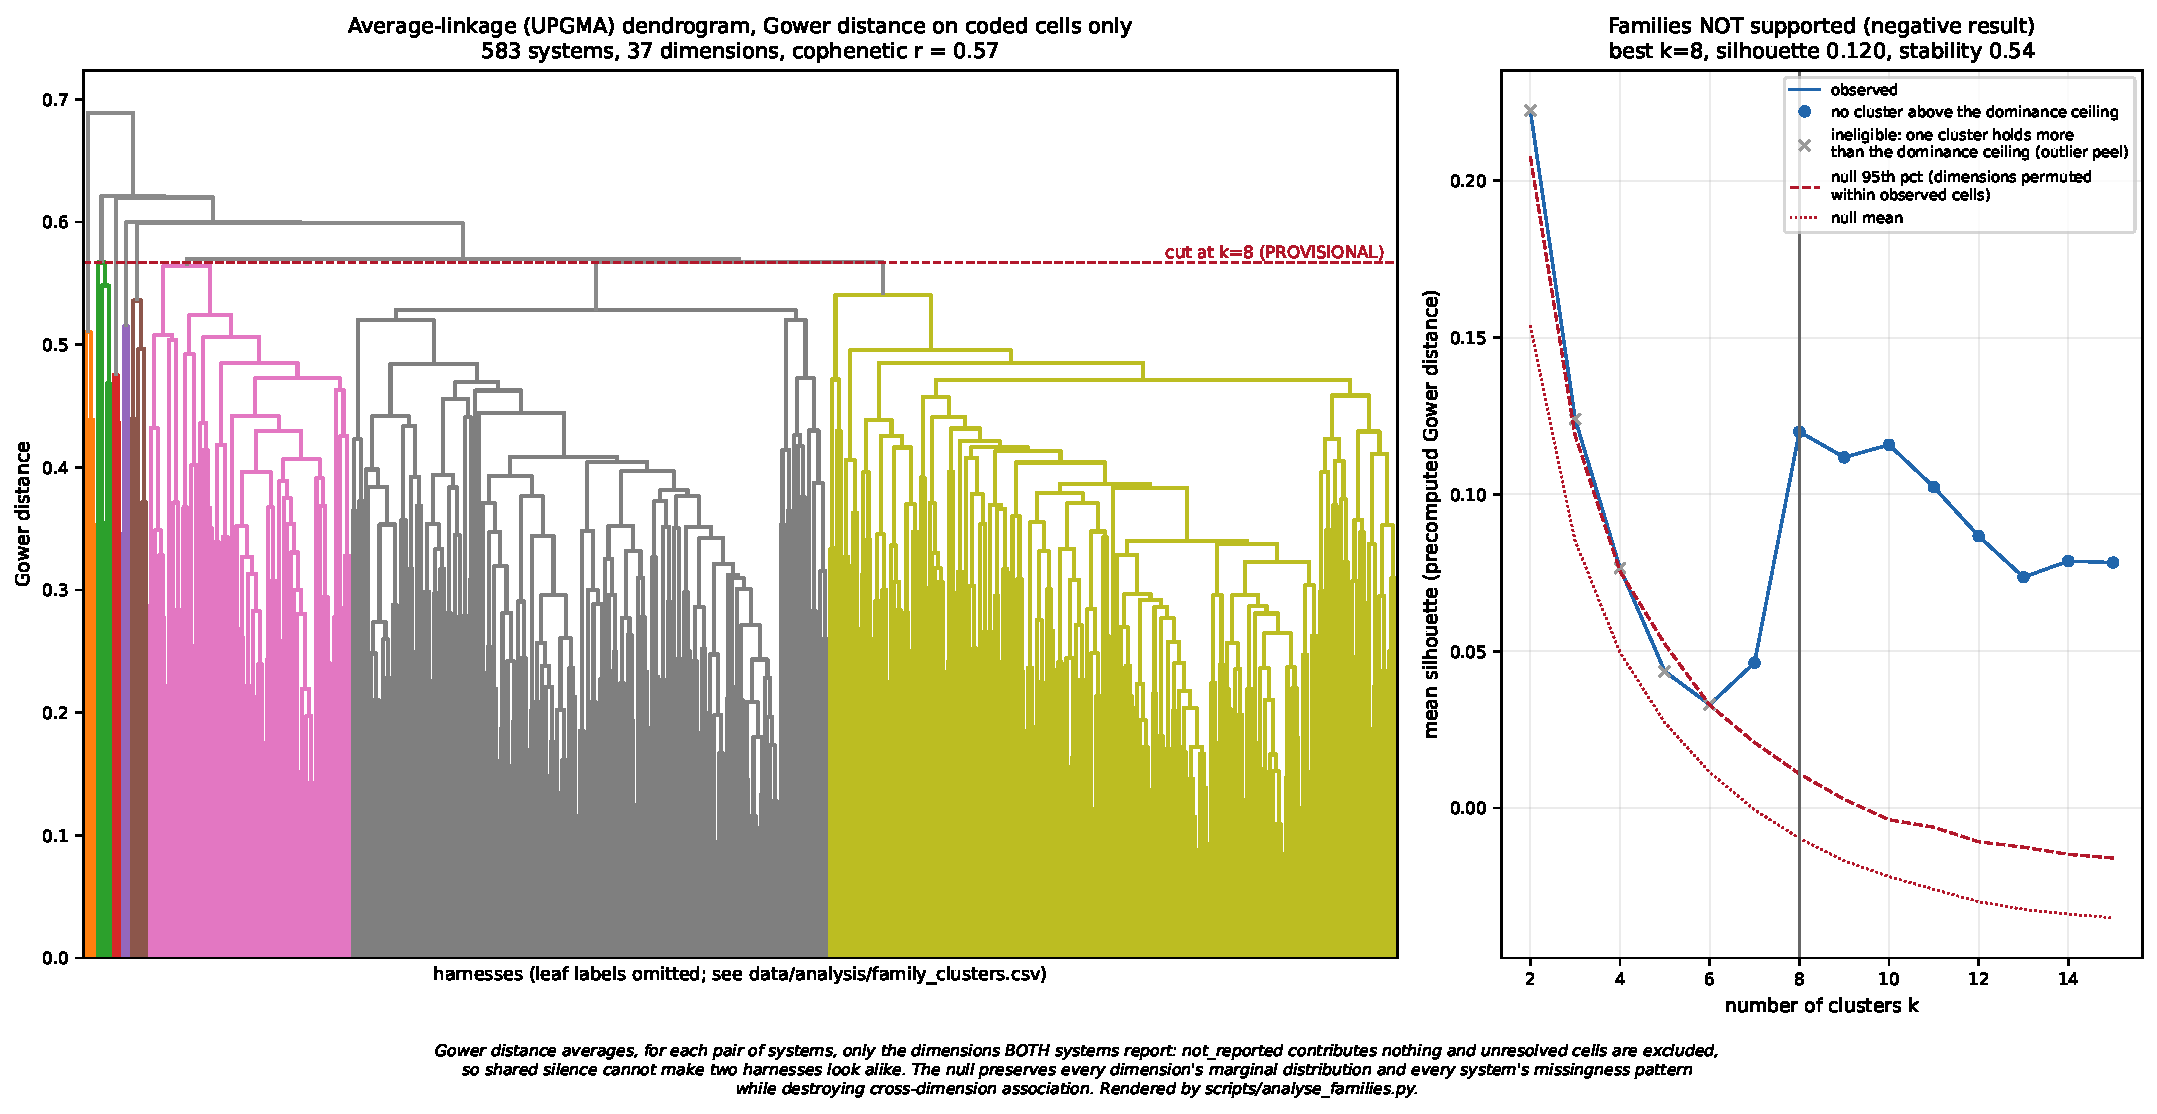
\includegraphics[width=\linewidth]{family_dendrogram}
\caption{Left: average-linkage dendrogram over the Gower distance, 583 systems, unweighted (cophenetic
correlation 0.571). Right: mean silhouette against $k$ beside the null's 95th percentile. The cut
$k = 8$ clears the null at 0.120 and misses the floor of 0.25: there is structure, but not enough to call families.}
\label{fig:landscape_dendrogram}
\end{figure}

The partition fails the silhouette \citep{rousseeuw1987silhouette} and stability
\citep{hennig2007stability} bars and passes the null, and the pass is what makes the failure informative
rather than inconclusive: because the null is maximized over $k$ as the data were, 0.120 is signal at a
selection-adjusted $p = 0.002$, yet below the 0.25 floor, and Figure~\ref{fig:landscape_dendrogram}
shows no $k$ that reaches it. No admissible linkage does better: weighted and complete linkage peak
lower, and single linkage never yields an eligible cut. Ward and centroid linkage were not run, because
they assume Euclidean coordinates that a Gower distance does not provide.

The alternative explanation, that clusters track documentation completeness rather than design, fails
for the clusters that carry any description. The three clusters holding at least 5\% of the set have
mean coded shares spanning 3.6 points. A Kruskal--Wallis test across all eight clusters does reject
equality ($H = 31.78$, $p = 4.5 \times 10^{-5}$), but it is driven by clusters of four to eight systems,
one of seven systems at 83.8\% and one of eight at 55.6\%.

Three regions are large enough to describe, and all three are provisional because the partition that
produced them failed its bars. The largest, 252 systems (43.2\%), is a subagent-spawning orchestrator,
with \texttt{subagent\_spawn} delegation in 77\% of members against 4\% elsewhere. The second, 212
systems (36.4\%), is the single-agent loop, with no delegation mechanism in 93\% against 13\%. The
third, 90 systems (15.4\%), is the pipeline and role-handoff design, with \texttt{role\_handoff} in 76\%
against 6\%. These are labels for regions of a continuum, not types, and membership is not a property
of a system.

Taxonomy papers in this area assert families of harness architecture
\citep{meng2026harnesssurvey,li2026harnessengineering,twodim2026agentpatterns}; on 583 systems, against
bars fixed before clustering, those families do not separate, and harness design reads as weakly coupled
choices rather than a few architectures.

\subsection{Design choices are weakly coupled, and shared silence manufactures the opposite impression}
\label{subsec:associations}

Once silence is removed, coupling between design dimensions is weak almost everywhere. For each pair we
computed a bias-corrected Cram\'er's V \citep{cramer1946methods,bergsma2013cramersv} on complete pairs,
the systems for which both dimensions carry a value, tested by permutation with 20,000 draws and
Benjamini--Hochberg correction \citep{benjamini1995fdr}. Of the 703 pairs, the 37 involving
\texttt{pinned\_version} are excluded; over the other 666, mean corrected V is 0.167
(Table~\ref{tab:landscape_assoc}). One pair exceeds 0.6: \texttt{multi\_agent\_topology} $\times$
\texttt{delegation\_mechanism}, at 0.720 on 841 systems ($q = 0.00026$), close to definitional because a
single-agent system has nothing to delegate to. The next-strongest, \texttt{protocol\_standardization}
$\times$ \texttt{rollback}, reaches 0.559 on only 140 systems.

\begin{table}[tbp]
\caption{Pairwise association under two treatments of silence over the 666 testable pairs, unweighted
(median 302 complete systems per pair, range 57--1,251). V: bias-corrected Cram\'er's V; significance: a
20,000-draw permutation test at Benjamini--Hochberg $q < 0.05$. Complete pairs are primary.}
\label{tab:landscape_assoc}
\footnotesize
\begin{tabular}{lrrr}
\toprule
Treatment of \texttt{not\_reported} & Mean V & Significant pairs & Significant only here \\
\midrule
Excluded (complete pairs)    & 0.167 & 385 & 2 \\
Counted as a level           & 0.168 & 648 & 265 \\
\bottomrule
\end{tabular}
\end{table}

Counting silence as a value manufactures structure. Table~\ref{tab:landscape_assoc} shows that treating
\texttt{not\_reported} as an ordinary level barely moves the mean V but raises the pairs significant at
BH $q < 0.05$ from 385 to 648 of 666, and 265 pairs are significant only under that treatment. Those 265 detect which
dimensions get documented together, not which designs co-occur; Supplement~S6 maps the change
pair by pair. The worst case is \texttt{tracing} $\times$
\texttt{eval\_hooks}: V is 0.000 on the 483 systems reporting both (permutation $p = 1.0$) and 0.241 at
$q = 0.00007$ once all 1,251 systems enter with silence counted as a value.

The caveat runs the other way. Complete pairs condition on joint reporting, which is not random, so if
silence hides a real association the complete-pair V misses it. Two pairs are significant only on
complete pairs, where counting silence dilutes an association the documented subset shows, and 20 more
keep their conclusion with a coefficient attenuated by shared silence. Both treatments are therefore
released in full in the replication package, with complete pairs primary.

With silence removed, harness design dimensions are close to independent apart from one near-definitional
pair. An analysis that treats \texttt{not\_reported} as a design choice will recover a correlation
structure made by who writes documentation, and with so little coupling to build on, the negative
clustering verdict of Section~\ref{subsec:families} is the expected outcome.

% Section 7 (RQ3). Every number that comes from the corpus-wide ablation harvest is a macro defined in
% tables/rq3_macros.tex, generated together with the three table fragments input below, so a rerun of
% the harvest updates this section without editing it. So are the two sensitivity analyses (the layer
% correlation before the mapping rules, the cross-paper headline without baseline-only keys). Numbers
% that do not come from that harvest (the other cross-paper contrasts, the coded-set harvest, the
% own-arm test, the attribution study, the pilot) are literals and are fixed.
% Macro formats this text assumes (all used in text mode, never inside $...$):
%   counts            plain numbers, thousands separator where needed (\rqCorpusContrasts -> 867)
%   *Pct              number only, no percent sign; the text appends \% (\rqSignSharePct -> 91)
%   \rqSVPooled, \rqSVDiscounted, \rqCoverageRho, \rqCoverageP   signed or plain decimal, text-safe
%   \rqPreRuleRho, \rqPreRuleP, \rqXPOtherEffect, \rqXPOtherP     likewise
%   \rqSVCIz, \rqSVPI, \rqXPOtherCI  interval including its brackets, text-safe ([$+0.107$, $+0.187$])
%   \rqZeroDimList, \rqPIExcludesZeroDims   \texttt names joined with commas and "and"
%   \rqZeroLayerList  layer letters joined with "and"; the word "empty" if the set is empty
%                     (the sentence reads "the set of layers with no ablated dimension is \rqZeroLayerList")
%   \rqHarvestTierCoverage   a noun phrase (e.g. "28\% of the top-signal tier and none of the second")
%   \rqHarvestDate    a date
%   \rqSignSharePct   share of the \rqSignDenom contrasts on POOLED dimensions (coded-set plus
%                     corpus-wide) that favour the component

\section{Design choices versus outcomes}\label{sec:outcomes}

Research question~3 asks which harness design choices are associated with better task outcomes.
Three designs can address it, and they differ in what each can identify
(Figure~\ref{fig:rq3-triangulation}). A cross-paper association compares coded systems inside a shared
benchmark, split and base model; measurement error on the design variable attenuates it towards zero,
while the choice of reference systems can inflate it. A within-study meta-analysis pools the ablations
authors publish about their own components; selective reporting inflates it, so its estimates are
\emph{upper bounds}. Only a controlled, compute-matched ablation identifies a component's effect at
equal compute. Table~\ref{tab:rq3-bounds} sets the three side by side with the direction of each
bound. \citet{guo2026qa2task} run the closest prior
analysis; they compare harnesses by identity, where we compare them by coded dimension.

\begin{figure}[t]
  \centering
  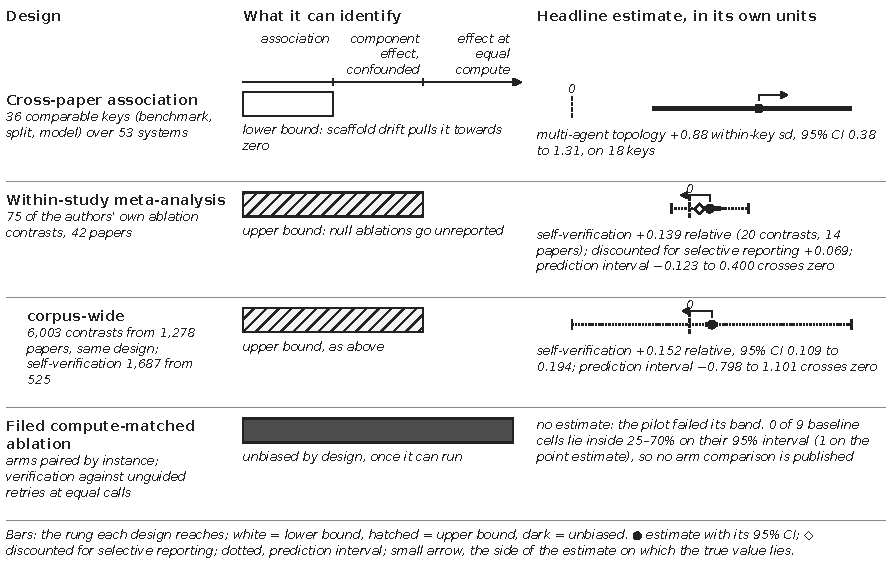
\includegraphics[width=\linewidth]{rq3_triangulation}
  \caption{The three RQ3 designs, placed by what each can identify. Cross-paper association within comparable keys (36 keys) can show only co-occurrence; scaffold drift biases it towards zero and baseline selection away from it, so the $+0.88$ within-key sd for multi-agent topology is a lower bound only against drift (Section~\ref{subsec:comparability}). The within-study meta-analysis of authors' own ablations identifies a component effect but is inflated by unreported nulls, so its pooled effects are upper bounds; the corpus-wide row pools \rqTotalContrasts{} contrasts from \rqTotalPapers{} papers under the same design. Only a controlled compute-matched ablation identifies the effect at equal compute; our filed one failed its pilot band, so the one design that could settle RQ3 has not yet produced an estimate.}
  \label{fig:rq3-triangulation}
\end{figure}

% RQ3 designs and their bounds
% GENERATED by scripts/make_rq3_tables.py - do not edit; re-run the script instead.
% sources (mtime, UTC):
%   paper/tables/outcomes_summary.json  (2026-09-25T15:27:23Z)
%   data/analysis/ablation_pooled_corpus.csv  (2026-09-25T16:13:00Z)
%   data/analysis/ablation_credible_corpus.csv  (2026-09-25T16:13:00Z)
%   data/analysis/ablation_summary_corpus.json  (2026-09-25T16:13:00Z)
%   data/tier3/pilot/pilot_summary.json  (2026-09-25T06:14:15Z)
%   data/tier3/pilot_v2/pilot_v2_summary.json  (2026-09-25T15:56:13Z)
%   schema/dimensions.json  (2026-09-25T14:21:14Z)
% generated: 2026-09-25T17:21:54Z
\begin{table}
\centering
\caption{Three designs for RQ3 and the direction of their bounds. The within-study and registered designs are shown for self-verification (E1), the one component all three measure; the cross-paper design shows its headline contrast (multi-agent topology (C3), the one that survives both the key bootstrap and the permutation test) and, beneath it, the focal dimension's own cross-paper value. The cross-paper estimate is a standardised within-key difference ($d$, in within-key SDs); the within-study estimate is a relative change. They are not on one scale; what they share is the direction in which each can be wrong.}
\label{tab:rq3-bounds}
\scriptsize
\setlength{\tabcolsep}{3pt}
\begin{tabular}{@{}p{0.10\linewidth}p{0.16\linewidth}p{0.15\linewidth}p{0.12\linewidth}p{0.12\linewidth}p{0.09\linewidth}p{0.14\linewidth}@{}}
\toprule
Design & Identifies & $n$ & Headline estimate & Interval (95\%) & Bound & Status \\
\midrule
% BEGIN ROWS
\raggedright Cross-paper association & \raggedright association between a coded design choice and standardised score across systems sharing benchmark, split and base model & \raggedright 18 keys, 38 systems (of 36 keys, 53 systems) & \raggedright multi-agent topology (C3): $d = +0.877$ within-key SD & \raggedright \ensuremath{[+0.379, +1.313]} (bootstrap over keys) & \raggedright lower for scaffold drift; in 7 of its 18 keys baseline selection can inflate it & \raggedright complete; detected; exact permutation $p = 0.0013$ \tabularnewline
\raggedright  & \raggedright  & \raggedright 3 keys, 11 systems & \raggedright self-verification (E1), executable checks vs none; fragile (3 keys): $d = -0.734$ within-key SD & \raggedright \ensuremath{[-1.414, -0.258]} (bootstrap over keys) & \raggedright lower (attenuated towards zero by scaffold drift) & \raggedright complete; not detected; exact permutation $p = 0.306$; fragile \tabularnewline
\raggedright Within-study meta-analysis & \raggedright the component's contribution inside the host systems whose authors ablated it & \raggedright 213 papers, 680 contrasts (all dimensions: 494 papers, 2{,}466 contrasts) & \raggedright self-verification (E1): $\hat\mu = +0.157$ (relative change) & \raggedright $z$ \ensuremath{[+0.132, +0.183]}; HK \ensuremath{[+0.131, +0.183]} & \raggedright upper (selective reporting) & \raggedright interim (harvest has read 96.7\% of the top-signal tier and none of the second); survives the bias discount ($z$ and HK) \tabularnewline
\raggedright Registered compute-matched ablation & \raggedright causal effect of the component at a matched model-call budget, on one suite and model & \raggedright pilot: 9 suite--model cells, arm A; revision: 48 runs, arms A and B; 93 instances needed at $\rho = 0.7$, 22 available & \raggedright not yet estimated & \raggedright --- & \raggedright unbiased (for that suite and model) & \raggedright filed, amendment pending; pilot failed its band; not runnable on available suites \tabularnewline
% END ROWS
\bottomrule
\end{tabular}
\end{table}


\subsection{Fewer than one coded system in twenty can be compared to a peer}\label{subsec:comparability}

The cross-paper design is nearly empty. Of the 1,256 coded systems the outcome analysis read, 646
report a benchmark score, but only 53 (4.2\%) share a canonical benchmark, split and base model with
another coded system, across 36 comparable keys. The registered mixed-effects regression was therefore
not fitted (amendment~11): its 38 design dimensions against 36 key clusters leave the coefficients
without support, and we report the non-fit rather than substitute an unregistered model.

Two of five contrasts, specified in amendment~11 after the comparable set was assembled, clear both of
their tests, and neither is free of selection.
Multi-agent topology is associated with $+0.88$ within-key standard deviations, 95\% bootstrap CI
$[+0.38, +1.31]$ over keys, on 18 keys and 38 systems, within-key permutation $p=0.0013$. It is an
association, not an effect, and two biases act on it in opposite directions. Scores do not name the
harness commit that produced them, while we code a pinned commit; that scaffold drift is measurement
error on the design variable and attenuates the estimate. Selection
pushes the other way: in \rqXPBaselineKeys{} of the 18 keys every reference system is a recurring
baseline harness, and on the other \rqXPOtherKeys{} keys the association is \rqXPOtherEffect{}
\rqXPOtherCI{} (permutation $p$ of \rqXPOtherP), so it is a lower bound only against drift, and its
detection rests on the baseline keys.

The other contrasts are reported with what they could have detected. \texttt{explicit\_plan} is a null,
$+0.36$ $[-0.30, +0.97]$, with a minimum detectable effect (MDE) of 1.05 within-key standard
deviations. \texttt{executable\_verification}, on 3 keys, has a bootstrap interval that excludes zero,
$-0.73$ $[-1.41, -0.26]$, but an exact permutation test that does not ($p=0.306$; MDE 1.87), so it is
read as a null. \texttt{any\_retry} varies inside only 2 keys, whose sign-symmetric label assignments
floor its two-sided $p$ at 0.500, so it is not estimable. \texttt{any\_compaction} clears both tests at
its design floor ($p=0.042$), but all 4 of its keys use a recurring baseline as reference, so it is
reported as confounded.

\emph{Takeaway.} The cross-paper literature supports one association, detected only with the keys
that compare against baselines, and cannot identify design effects, a measured property of how the
field reports results.

\subsection{Authors' own ablations barely separate design dimensions}\label{subsec:ablations}

The within-study design pools authors' published ablations of their own systems. Each contrast is one
codebase at one commit with one base model, differing in one component, and its effect is the relative
change $(\text{with}-\text{without})/\text{with}$ in the paper's own metric. Beyond the
\rqCodedContrasts{} coded-set contrasts from \rqCodedPapers{} papers, the completed extraction stage
read the full text of \rqCorpusPapersExtracted{} included papers, \rqHarvestTierCoverage{} of a
prefilter that ranks papers by ablation content, and added \rqCorpusContrasts{} pool-eligible contrasts from \rqCorpusPapersWithContrast{}
papers. \rqPoolableDims{} dimensions now reach the three papers needed to pool, against 8 on the
coded set alone.

Rows enter the pool only under fixed rules. A row is kept if its two scores appear together and
verbatim, share a scale and metric, vary the harness rather than the model, and map to a design
dimension above a confidence floor. Seven mapping rules then correct attributions the text
contradicts: a removed sandbox that takes code-execution feedback with it is self-verification, not
isolation, and a row whose scores run together, report a delta, or carry a label that contradicts its
direction is dropped. Every firing is logged in the replication package.

% RQ3 pooled ablations
% GENERATED by scripts/make_rq3_tables.py - do not edit; re-run the script instead.
% sources (mtime, UTC):
%   data/analysis/ablation_pooled_corpus.csv  (2026-09-25T16:13:00Z)
%   data/analysis/ablation_credible_corpus.csv  (2026-09-25T16:13:00Z)
%   data/analysis/ablation_summary_corpus.json  (2026-09-25T16:13:00Z)
%   schema/dimensions.json  (2026-09-25T14:21:14Z)
% generated: 2026-09-25T16:13:01Z
\begin{table}
\centering
\caption{Within-study meta-analysis of published ablations, coded-set and corpus-wide harvests combined (harvest snapshot of 25 September 2026; the harvest is incomplete). One row per design dimension with contrasts from at least 3 papers (18 dimensions; 6 more have contrasts from fewer papers and are not pooled). Effect: relative change $(\mathrm{with}-\mathrm{without})/\mathrm{with}$ on the paper's own metric, $+$ = the component helped. $\hat\mu$: DerSimonian--Laird random-effects mean over paper-level effects; 95\% CI by the normal ($z$) and Hartung--Knapp (HK) methods; 95\% PI: prediction interval for a new host system, \textbf{bold} where it excludes zero. Discounted $\hat\mu$ applies the dimension's own publication-bias discount. \emph{Surv.}: the discounted lower CI bound still exceeds 0.02 and trim-and-fill keeps the sign, judged on the $z$ / HK bound. Papers: total (coded-set + corpus-wide). Every estimate is an \emph{upper} bound on the component's contribution: authors report the ablations that favour their component.}
\label{tab:ablations}
\footnotesize
\setlength{\tabcolsep}{2.5pt}
\begin{tabular}{@{}p{0.2\linewidth}rrrcccrrc@{}}
\toprule
 & & & \multicolumn{7}{c}{relative change, $+$ = component helped} \\
\cmidrule(l){4-10}
Dimension & Papers & Contr. & $\hat\mu$ & 95\% CI ($z$) & 95\% CI (HK) & 95\% PI & $I^2$ (\%) & Disc.\ $\hat\mu$ & Surv.\ $z$/HK \\
\midrule
% BEGIN ROWS
\raggedright Self-verification (E1) & 213 (14+201) & 680 & \ensuremath{+0.157} & \ensuremath{[+0.132,+0.183]} & \ensuremath{[+0.131,+0.183]} & \ensuremath{[-0.172,+0.487]} & 91.7 & \ensuremath{+0.082} & yes/yes \tabularnewline
\raggedright Long-term memory (D2) & 133 (4+131) & 455 & \ensuremath{+0.151} & \ensuremath{[+0.125,+0.176]} & \ensuremath{[+0.123,+0.179]} & \ensuremath{[-0.095,+0.397]} & 77.3 & \ensuremath{+0.080} & yes/yes \tabularnewline
\raggedright Planning granularity (C2) & 86 (4+83) & 245 & \ensuremath{+0.161} & \ensuremath{[+0.126,+0.197]} & \ensuremath{[+0.127,+0.196]} & \ensuremath{[-0.128,+0.451]} & 81.6 & \ensuremath{+0.085} & yes/yes \tabularnewline
\raggedright Repo/environment context strategy (A2) & 85 (5+80) & 253 & \ensuremath{+0.177} & \ensuremath{[+0.129,+0.226]} & \ensuremath{[+0.128,+0.227]} & \ensuremath{[-0.241,+0.596]} & 90.4 & \ensuremath{+0.090} & yes/yes \tabularnewline
\raggedright Multi-agent topology (C3) & 79 (6+74) & 272 & \ensuremath{+0.174} & \ensuremath{[+0.130,+0.218]} & \ensuremath{[+0.129,+0.219]} & \ensuremath{[-0.181,+0.530]} & 88.6 & \ensuremath{+0.090} & yes/yes \tabularnewline
\raggedright Loop primitive(s) (C1) & 52 (1+51) & 156 & \ensuremath{+0.192} & \ensuremath{[+0.139,+0.245]} & \ensuremath{[+0.148,+0.236]} & \ensuremath{[-0.163,+0.547]} & 87.6 & \ensuremath{+0.099} & yes/yes \tabularnewline
\raggedright Short-term state (D1) & 30 (3+28) & 59 & \ensuremath{+0.206} & \ensuremath{[+0.108,+0.304]} & \ensuremath{[+0.098,+0.314]} & \ensuremath{[-0.330,+0.742]} & 91.6 & \ensuremath{+0.104} & yes/yes \tabularnewline
\raggedright Tool count at pinned version (B2) & 27 (4+23) & 95 & \ensuremath{+0.173} & \ensuremath{[+0.017,+0.328]} & \ensuremath{[+0.079,+0.267]} & \ensuremath{[-0.675,+1.021]} & 97.9 & \ensuremath{+0.087} & no/yes \tabularnewline
\raggedright Context compaction (A3) & 19 (4+15) & 43 & \ensuremath{+0.085} & \ensuremath{[+0.048,+0.122]} & \ensuremath{[+0.046,+0.124]} & \textbf{\ensuremath{[+0.029,+0.141]}} & 5.2 & \ensuremath{+0.052} & yes/yes \tabularnewline
\raggedright Delegation mechanism (C4) & 14 (1+13) & 42 & \ensuremath{+0.087} & \ensuremath{[-0.024,+0.197]} & \ensuremath{[-0.047,+0.221]} & \ensuremath{[-0.355,+0.528]} & 89.4 & \ensuremath{+0.002} & no/no \tabularnewline
\raggedright Observation formatting (A4) & 14 (1+13) & 37 & \ensuremath{+0.169} & \ensuremath{[+0.061,+0.277]} & \ensuremath{[+0.081,+0.257]} & \ensuremath{[-0.258,+0.596]} & 90.5 & \ensuremath{+0.087} & yes/yes \tabularnewline
\raggedright System-prompt style (A1) & 12 (1+11) & 31 & \ensuremath{+0.138} & \ensuremath{[+0.048,+0.227]} & \ensuremath{[+0.004,+0.272]} & \ensuremath{[-0.153,+0.428]} & 71.6 & \ensuremath{+0.067} & yes/no \tabularnewline
\raggedright Retry policy (E2) & 12 (1+11) & 23 & \ensuremath{+0.084} & \ensuremath{[+0.041,+0.128]} & \ensuremath{[+0.035,+0.133]} & \ensuremath{[-0.032,+0.201]} & 47.1 & \ensuremath{+0.046} & yes/no \tabularnewline
\raggedright Rollback / undo (E3) & 8 (1+7) & 21 & \ensuremath{+0.066} & \ensuremath{[-0.004,+0.137]} & \ensuremath{[-0.019,+0.151]} & \ensuremath{[-0.116,+0.249]} & 45.1 & \ensuremath{+0.037} & no/no \tabularnewline
\raggedright Guardrails (H4) & 7 (0+7) & 8 & \ensuremath{+0.107} & \ensuremath{[+0.069,+0.145]} & \ensuremath{[+0.067,+0.147]} & \textbf{\ensuremath{[+0.058,+0.157]}} & 0.0 & \ensuremath{+0.085} & yes/yes \tabularnewline
\raggedright Edit primitive (B3) & 4 (0+4) & 11 & \ensuremath{+0.169} & \ensuremath{[+0.042,+0.295]} & \ensuremath{[-0.046,+0.384]} & \ensuremath{[-0.261,+0.599]} & 34.8 & \ensuremath{+0.084} & yes/no \tabularnewline
\raggedright Termination condition (F1) & 4 (0+4) & 9 & \ensuremath{-0.007} & \ensuremath{[-0.025,+0.010]} & \ensuremath{[-0.018,+0.003]} & \ensuremath{[-0.045,+0.031]} & 0.0 & \ensuremath{-0.007} & no/no \tabularnewline
\raggedright Tracing (H1) & 3 (0+3) & 6 & \ensuremath{+0.052} & \ensuremath{[-0.050,+0.154]} & \ensuremath{[-0.151,+0.255]} & \ensuremath{[-1.014,+1.118]} & 46.1 & \ensuremath{+0.002} & no/no \tabularnewline
% END ROWS
\bottomrule
\end{tabular}
\end{table}


Table~\ref{tab:ablations} gives the pooled result, and its central fact is convergence. Most
dimensions show a positive relative gain of similar size: surviving gains span
\rqEffectRangeSurviving{}, their middle half \rqEffectIQRSurviving, and most intervals overlap.
Context compaction has the lowest surviving gain and the least heterogeneity of the well-populated
rows; its $z$ interval lies below those of multi-agent topology and loop primitives but overlaps the
other four best-populated dimensions. Short-term state, as well populated, pools near zero. The bias
signature repeats: \rqSignSharePct\% of the \rqSignDenom{} contrasts on pooled dimensions favour the
authors' component, heterogeneity is mostly high, and all \rqPIIncludesZeroCount{} prediction
intervals include zero.

Gains of one size from components this different fit one reporting filter better than coincidence:
an ablation is written up to show that a component helps. Misassigned labels would also pull rows
together, so convergence shows how little these ablations separate dimensions, not why.

The pre-stated discount rule fails to discriminate at this scale. The rule
shrinks each pooled effect by the larger of its own trim-and-fill and one-null-per-contrast shrinkage
\citep{duval2000trimfill,copas2000funnel}, and admits a dimension whose discounted confidence-interval
lower bound still clears 2\% relative. Of \rqPoolableDims{} dimensions, \rqDiscountSurviveZ{} pass, and
\rqDiscountSurviveHK{} pass with a Hartung--Knapp interval in place of the $z$ interval. The cause is
structural. For most positive effects the discount sits near one half (median \rqMedianDiscountPct\%), so
the rule reduces to asking whether an interval clears zero, and more contrasts make that easier
whatever produced the effect. On the coded set, with 3 to 14 papers per dimension, the same rule
admitted two dimensions; its selectivity there was a property of small samples.

The prediction-interval criterion \citep{higgins2009predictioninterval} is the secondary we can defend,
and it admits no dimension. A prediction interval clears zero only where between-paper heterogeneity is small, so the criterion asks
whether the next published ablation would also favour the component.

Self-verification's estimate is stable and no longer distinguished. On the coded set it pooled to at
most $+0.139$ on 14 papers ($+0.069$ after the discount); corpus-wide it pools to \rqSVPooled, 95\% CI
\rqSVCIz, on \rqSVPapers{} papers, with a prediction interval of \rqSVPI{} that includes zero, and
discounts to \rqSVDiscounted{} under one unreported null per contrast. A filtered literature produces
that stability as readily as a real effect does. The defensible sentence is that self-verification is worth at most about
\rqSVDiscounted{} relative in published ablations, and a sentence of the same form can be written for
most of the table.

Every estimate in Table~\ref{tab:ablations} is an upper bound. The within-study design absorbs four of
the five benchmark caveats we document, because both arms share one codebase, commit and team; what
survives is self-reporting, concentrated: each contrast is an author reporting on a component they
built.

\emph{Takeaway.} Authors' own ablations bound most components from above and rank almost none:
whatever is ablated appears to help by about the same amount, which fits selective reporting better
than equal real effects.

\subsection{Publication bias, measured on the sign distribution}\label{subsec:bias}

Selective reporting is measured here rather than assumed, and the measurement is the sign distribution.
Of the \rqSignDenom{} coded-set and corpus-wide contrasts on pooled dimensions, \rqSignSharePct\% favour
the authors' own component. The share does not rest on
our orientation of the metrics: \rqPolarityAssumedN{} contrasts take higher-is-better by assumption
because their metric names no direction, yet \rqPolarityStatedFavourPct\% of the
\rqPolarityStatedN{} with a stated direction favour the component (\rqPolarityAssumedFavourPct\% of the
rest). No rule reads an effect's sign, but the rule that drops a row whose label contradicts
its direction removed \rqDCLDropped{} rows (\rqDCLAgainst{} unfavourable as extracted); kept, they
would give \rqSignShareWithDCLPct\%. A component that helped only sometimes would produce more
dissent than that, and this distribution is the empirical warrant for reading
Table~\ref{tab:ablations} as upper bounds.

The within-paper baseline tables corroborate the mechanism; they are not a second measurement of it.
Over all 75 blocks containing the authors' own arm, from 37 papers, the own arm's advantage over chance
is not established (paper-clustered $p=0.21$). It survives only in tables of five or more arms, 14 of
17 against 6.95 expected ($p=4.4\times10^{-4}$), and those tables hold 70 of the 89 own-ablation arms:
large arm tables here are largely the paper's own ablation tables.

Egger's test \citep{egger1997bias} is reported but not leaned on: its input is partly our own
construction. Papers publish no standard errors, so a contrast's variance is reconstructed binomially
from its arm scores where the metric is a proportion, and set by an assumed 10\% relative standard
error for the other \rqVarAssumedN{} contrasts on pooled dimensions. Under that reconstruction,
at a given with-component score, the variance of the relative effect falls as the effect grows, so
random-effects weights \citep{dersimonian1986meta} favour the largest effects, pushing pooled estimates
upward as the upper bound declares, and the funnel tilts against small-study asymmetry, biasing
Egger's test towards non-detection.

\emph{Takeaway.} Author selection of what to publish is present at the magnitude the sign distribution
measures, and it acts on which contrasts reach print.

\subsection{Where the field ablates}\label{subsec:coverage}

Ablation density falls as a layer's silence rises. Table~\ref{tab:coverage} sets the harvested contrasts
against each layer's weighted \texttt{not\_reported} rate from the landscape analysis. Across the eight
substantive layers, the rank correlation between
silence and ablation density is Spearman's $\rho$ of \rqCoverageRho, exact one-sided permutation $p$ of
\rqCoverageP. On the coded set, layers F, G and H (budget and termination, sandbox and environment,
observability and governance) carried no ablation at all. The corpus-wide harvest reaches four of their
dimensions, through 1 to 21 papers each: termination condition (F1) pools to a precise null,
$-0.003$ $[-0.019, +0.014]$ with $I^2 = 0$, and guardrails (H4) to $-0.100$ with an interval spanning
zero, but \rqZeroDimCount{} dimensions still carry no published ablation (\rqZeroDimList), and the set
of layers with no ablated dimension is \rqZeroLayerList{}.

The mapping rules produce that empty layer but not the gradient. Of the \rqPreRuleGContrasts{}
contrasts the harvest first attributed to the sandbox layer, the rules reassigned
\rqPreRuleGRemapped{}, removals of code-execution feedback or file-system tools, to the dimensions they
take away (\rqPreRuleGRemapList), and dropped \rqPreRuleGDropped{}: \rqPreRuleGDroppedUnread{} with
unreadable scores and \rqPreRuleGDroppedUnnamed{} naming no isolation boundary or authorization. With
all seven rules undone $\rho$ is unchanged, \rqPreRuleRho{} (exact $p$ of \rqPreRuleP).

% RQ3 ablation coverage
% GENERATED by scripts/make_rq3_tables.py - do not edit; re-run the script instead.
% sources (mtime, UTC):
%   data/analysis/ablation_coverage_by_layer.csv  (2026-09-25T16:01:11Z)
%   data/analysis/ablation_coverage_summary.json  (2026-09-25T16:01:11Z)
%   data/analysis/ablation_coverage_by_layer_corpus.csv  (2026-09-28T13:53:57Z)
%   data/analysis/ablation_coverage_summary_corpus.json  (2026-09-28T13:53:57Z)
%   schema/dimensions.json  (2026-09-25T14:21:14Z)
% generated: 2026-09-28T13:53:57Z
\begin{table}
\centering
\caption{Ablation coverage by layer against layer silence (weighted share of systems whose dimension is \emph{not reported}). \emph{Coded-set}: contrasts harvested from the coded systems' outcome extraction; \emph{corpus-wide}: coded-set plus the full-text harvest, de-duplicated. Dimension and density columns are corpus-wide. $^\dagger$Layer M (metadata) cannot be ablated and is excluded from $\rho$. Still without a single published ablation: 7 of 31 ablatable dimensions (cost controls (F2), evaluation hooks (H3), execution isolation (G1), filesystem access (G2), network policy (G3), permission model (G4) and replayability (H2)). Absence of evidence about the literature, not evidence that those components do not matter.}
\label{tab:coverage}
\footnotesize
\begin{tabular}{@{}lrrrrrr@{}}
\toprule
 & Weighted & & Dims $\geq$1 & Contrasts & Contrasts & Contrasts \\
Layer & silence & Dims & contrast & (coded-set) & (corpus-wide) & per dim \\
\midrule
% BEGIN ROWS
A Context assembly & 40.2\% & 4 & 4 & 13 & 924 & 231.0 \\
B Tool interface & 71.4\% & 5 & 5 & 5 & 272 & 54.4 \\
C Control loop & 24.9\% & 5 & 5 & 26 & 1{,}651 & 330.2 \\
D Memory and state & 63.3\% & 3 & 3 & 8 & 1{,}263 & 421.0 \\
E Verification and repair & 60.9\% & 3 & 3 & 23 & 1{,}817 & 605.7 \\
F Budget and termination & 65.1\% & 3 & 2 & 0 & 29 & 9.7 \\
G Sandbox and environment & 81.6\% & 4 & 0 & 0 & 0 & 0.0 \\
H Observability and governance & 72.8\% & 4 & 2 & 0 & 47 & 11.8 \\
M Meta$^\dagger$ & 34.6\% & 7 & 0 & 0 & 0 & 0.0 \\
% END ROWS
\midrule
\multicolumn{7}{@{}l}{Spearman $\rho$, silence vs.\ corpus-wide density (layers A--H): $\rho = -0.738$, exact one-sided $p = 0.023$} \\
\multicolumn{7}{@{}l}{(40{,}320 permutations); coded-set density only: $\rho = -0.854$, $p = 0.0065$} \\
\bottomrule
\end{tabular}
\end{table}


This is an absence of evidence and is read as one: no paper in the harvest published a number for
removing these components, which says nothing about whether they matter. The layers that govern safe
deployment are the layers the literature has measured least.

\emph{Takeaway.} The field ablates the layers that describe what a harness does and seldom the layers
that bound it.

\subsection{Papers compare their system against its own configurations}\label{subsec:attribution}

The within-paper baseline table should have been RQ3's strongest design, and it fails for a reason
that is itself a finding. A block, one paper by benchmark by split by metric by model, holds
team, protocol and base model fixed. Yet 784 of the 819 comparator arms in the 324 estimable blocks
(95.7\%) cannot be tied to any system in the 6,504-system census, and the only 7 blocks with two or
more attributed comparators come from one paper, so no contrast in this design is replicated across
papers.

Name recall is not the explanation. A vetted alias table,
accepting a mapping only when the candidate's name is corroborated in that paper's own full text,
raised attributed comparator arms from 28 to 35 and left the number of blocks spanning more than one
paper unchanged. Of the 172 comparator labels the first reading judged to name a harness, 149 were
the reporting paper's own system under an abbreviation, such as \texttt{OH CodeActAgent v1.5} in the
OpenHands paper \citep{wang2024openhands}.

\emph{Takeaway.} Harness-to-harness comparison is largely not attempted; baseline
tables hold the paper's configurations and bare model names, a gap
\citet{samemodel2026harness} and \citet{scaffoldeffect2026} document from the model's side.

\subsection{Our own controlled ablation: filed, piloted, not yet run}\label{subsec:tier3}

Both published designs are author-reported, so before collecting any data we filed a controlled
ablation of our own as a protocol amendment, pending acceptance (Figure~\ref{fig:tier3-design}).
It targets self-verification, chosen when the coded-set harvest singled it out. A verification step
issues extra model calls, so every published contrast asks whether verifying helps, confounded with
compute, and never whether verifying and repairing beats unguided retrying at equal compute. Arm~C
therefore receives exactly the calls arm~B used, matched per instance rather than on average. No paper
among the 42 coded-set papers that publish a component ablation runs such a control, a distinction
that work on feedback compute makes salient \citep{efc2026scaling}.

\begin{figure}[t]
  \centering
  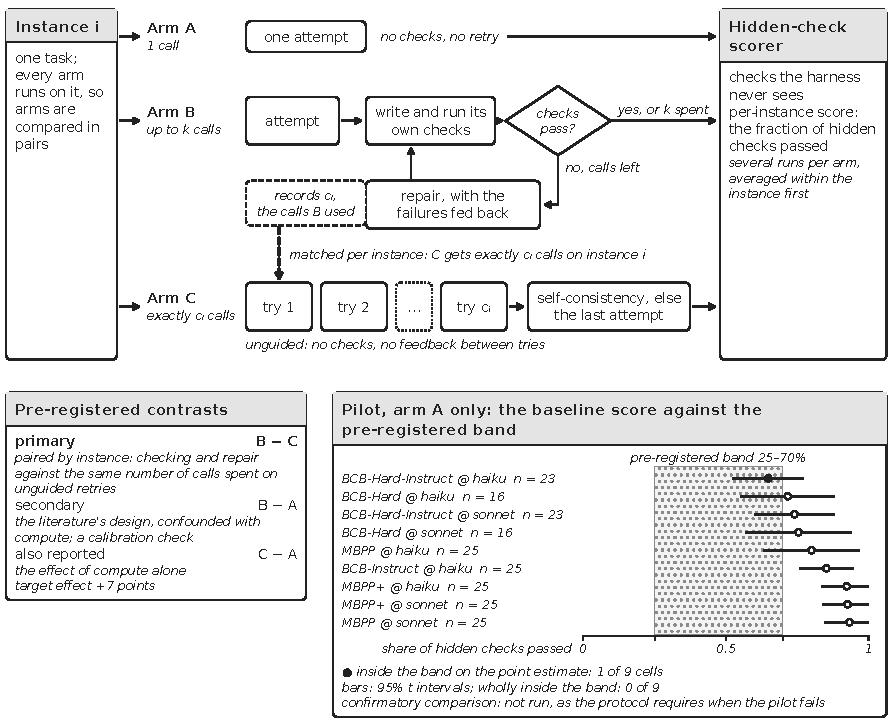
\includegraphics[width=\linewidth]{tier3_design}
  \caption{The filed compute-matched ablation, drawn for one instance. Arm~A makes a single call. Arm~B attempts, runs checks it wrote itself and repairs until they pass or $k$ calls are spent, recording the calls it used, $c_i$. Arm~C then receives exactly $c_i$ independent, unguided attempts on the same instance. The primary contrast, $B - C$ paired by instance, separates what verification does with its calls from how many calls it spends, which is the confound in every published self-verification ablation. Inset: the arm-A pilot against the pre-stated 25--70\% band. One of nine suite--model cells lies inside the band on its point estimate and none on its 95\% interval, so under the pre-stated rule no arm comparison is published.}
  \label{fig:tier3-design}
\end{figure}

The pilot failed its pre-stated band, so no arm comparison is published. The suite was to be chosen
on a disjoint pilot pool by arm-A accuracy in the 25--70\% band, read on the mean fraction of hidden
checks passed, and eight of the nine suite--model cells sit above the ceiling
(Figure~\ref{fig:tier3-design}, inset). The one inside, the Instruct presentation of BigCodeBench-Hard
with the smaller of the two generators, fails twice over: its interval
crosses the ceiling and cannot be resolved on a 23-instance pilot pool, and its confirmatory pool falls
far short of the 93 instances the analysis plan requires (Table~\ref{tab:rq3-bounds}). The full
Instruct split, which has the instances, sits entirely above the ceiling. Four of the nine cells are in
band on the binary secondary measure; we did not substitute it for the primary one.

One single-arm, descriptive pilot measurement is reportable. Across 56 arm-B diagnostic runs, a harness
that writes, runs and repairs against its own checks accepted its first attempt 50 times, at a mean of
1.16 calls, and three of those 50 scored 0.00 against the hidden tests. Model-written verification
mostly does not fire, and when it passes it can be blind to total failure, which bears on the mechanism
the published contrasts credit without contradicting their upper bound.

Where arm~B declines to spend its budget, arm~C is matched to a single call, and on those instances the
paired contrast carries no information about verification. A revision of the design, filed as a dated
amendment, removes that option: arm~B runs four verify-and-repair rounds whether or not its own checks
pass, and the estimand is conditioned on the stratum in which the treatment fires, defined by arm~A
rather than by arm~B's own outcome so that the conditioning cannot bias the contrast against~B. Its
pilot, on arms A and~B with the smaller generator, shows the redefinition works: the forced rounds
changed the submitted code in 17 of 48 runs, while the original arm accepted its first attempt in 41 of
48, three of them scoring 0.00 on the hidden tests.

The revision also exposed a defect that leaves the verdict unchanged. Pilot and confirmatory pools had
been separated by suite name rather than by task, so 12 of the in-band cell's 34 confirmatory tasks had
already been piloted under another presentation. Separated by task, 22 clean instances remain against
the 93 required; assuming the two arms' instance means correlate at 0.7, the smallest effect 22
instances can detect is 0.149 on the continuous score, over twice the planned 7 points. The design is
sound and still unrunnable on the suites available.
% TIER3V2-HOOK (filled 2026-09-25 from the amendment 12a pilot)

\emph{Takeaway.} The compute-matched question that would turn Section~\ref{subsec:ablations}'s upper
bounds into an unconfounded estimate is filed and unanswered.

% TODO: the protocol amendment for the compute-matched ablation is filed but not yet accepted at the
% registry. When it is, give it its number and date in the first paragraph of this subsection, in the
% amendments table of the supplement, and in the PRISMA checklist.

\section{The reporting deficit and what would close it}
\label{sec:open}

Two things follow from the measurements above: a change the field can make now at no research cost, and
three questions that need experiments nobody has run.

\subsection{A reporting checklist, taken from where the silence is}
\label{subsec:checklist}
\label{subsec:record}

The silence is concentrated enough to be addressed by a list. The twelve dimensions with the highest
weighted \texttt{not\_reported} rate all sit above 76\%, and nine of the twelve describe how a harness is
bounded or recovered; tool count, protocol standardization, and context compaction are the exceptions.
Each becomes a minimum statement: Table~\ref{tab:checklist} gives the five most silent, and
Supplement~S6 all twelve. Each item is
one sentence or configuration line, needs no experiment, and is checkable against the released
artifact; that separates a reporting item from a recommendation.

A negative answer satisfies an item as fully as a positive one, which makes the list cheap to adopt.
``The agent runs in the host shell with no isolation and no network restriction'' answers two rows, and
our scheme codes it as a value rather than as silence. Without such a sentence, neither a reader nor our
coder can tell an unbounded system from an undocumented one. A general call to state the harness exists
\citep{zhang2026harnessreporting}. The audit adds which items go unstated and how often, weighted to the
census, and the list is short because the measurement made it short.

The same gap sits one level up: no board in our harvest of 4,887 leaderboard entries records which
harness commit produced a score. Answering the twelve items would not make harnesses comparable. It
would let a reader see how a system is bounded, and give a design analysis dimensions stated often
enough to use.

\begin{table}[t]
\caption{The five items of the reporting checklist with the highest weighted silence rate; all twelve
are in Supplement~S6. \emph{Silent} is the weighted census share of systems whose sources say nothing
about the dimension (design standard errors in Table~\ref{tab:landscape_layers}), an upper bound
(\S\ref{subsec:humanaudit}). The rates measure
documents, not systems.}
\label{tab:checklist}
\footnotesize
\begin{tabular}{llrp{0.50\linewidth}}
\toprule
Layer & Dimension & Silent & Minimum a paper or repository should state \\
\midrule
G & \texttt{network\_policy} & 93.3\% & Whether the agent can reach the network during a run, and if so what is reachable: open egress, an allowlist, or nothing. \\
H & \texttt{replayability} & 90.6\% & Whether a finished run can be replayed from stored artifacts, and whether fully, from inputs only, or not at all. \\
G & \texttt{filesystem\_access} & 87.5\% & The writable scope: the whole host, one working directory, a copy-on-write overlay, or read-only. \\
E & \texttt{rollback} & 86.4\% & What happens to partial edits when a step fails: snapshot restore, version-control revert, or nothing. \\
D & \texttt{state\_persistence} & 86.2\% & Whether a run can be resumed after interruption, and from what: full state, a checkpoint, or nothing. \\
\bottomrule
\end{tabular}
\end{table}

\subsection{Three open questions}
\label{subsec:openq}

\textbf{Does self-verification help at equal compute?} The pooled ablation effect is an upper bound,
\rqSVPooled{} relative on the completed corpus-wide harvest before its bias discount and about
\rqSVDiscounted{} after it, and its prediction interval, \rqSVPI, includes zero. It is also no longer
distinguished: most poolable dimensions show a gain of similar size, so published ablations cannot say
whether verification matters more than any other component. Verification issues extra model calls,
and none of the 42 coded-set papers that ablate a component runs a compute-matched control, so the
ablations cannot separate design from compute. A three-arm
study would: one attempt; verify-and-repair up to $k$ calls; and the same calls, per instance, spent on
unguided retries. We froze that design on 2026-09-24 and filed it, with a dated revision, as protocol
amendments, now accepted at OSF; only pilot data exist, and no available suite supplies the 93
in-band instances it needs.

\textbf{Do the components that bound an agent matter?} Almost nobody has published a number. On the
coded-set harvest, none of the eleven dimensions of layers F, G, and H carried a usable ablation contrast
across the 42 papers that ablate anything. The corpus-wide harvest reaches four of them, where
termination condition pools to a precise null and guardrails to an interval spanning zero; of the
\rqPreRuleGContrasts{} contrasts it first attributed to layer G, \rqPreRuleGRemapped{} removed
code-execution feedback or file-system tools, not a sandbox or a permission policy, and the other
\rqPreRuleGDropped{} were unreadable or named no sandbox mechanism. Under the
fixed mapping rules of Section~\ref{sec:outcomes}, \rqZeroDimCount{} of the
\rqAblatableDimCount{} ablatable dimensions carry none (\rqZeroDimList). That is an absence of evidence about the literature, not evidence that the components are
harmless to remove.
The nearest controlled measurement varies scaffold architecture rather than a bound and gives the
model no tools: over 62,808 scored evaluations, scaffold architecture explains 0.4\% of the variation
in measured safety and benchmark choice 19.3\% \citep{safetyscaffolding2026}.
The closing study is small: one harness, one task suite, and a bound varied one level
at a time. Its tasks should include ones the bound exists to block, so the bound's cost and the
failure it prevents appear together.

\textbf{Do design families exist in a better-reported corpus?} Ours does not contain them: the best
eligible clustering reached a mean silhouette of 0.120 against a pre-stated floor of 0.25. That result
covers only the half of the corpus reporting enough to be clustered, and \S\ref{subsec:construct} gives a
second explanation our cells cannot rule out. The identical procedure, run on a corpus that answers
the twelve-item checklist as a condition of inclusion and coded with a loop-driver axis, would separate
the two.

\section{Threats to validity}
\label{sec:threats}
% Former subsection labels, kept so that existing cross-references resolve to this section; their
% content is now a row of Table~\ref{tab:threats}.
\label{subsec:rule5}\label{subsec:loop}\label{subsec:weights}\label{subsec:benchmarks}
\label{subsec:ourablation}\label{subsec:searchbias}\label{subsec:searchfreeze}\label{subsec:lessons}

Table~\ref{tab:threats} gives each threat's direction, the mitigation performed, and what
that mitigation leaves unestablished; several are weaker than we would have chosen. Three threats bound
the conclusions and are discussed below.

\begin{table}[tp]
\caption{Threats to validity. \emph{Direction} is the effect on the estimate named in the cell.
\emph{Mitigation} lists only checks that were performed. Row groups: review process; sample and search;
evidence base; taxonomy.}
\label{tab:threats}
\footnotesize
\begin{tabular}{@{}p{0.17\linewidth}p{0.10\linewidth}p{0.38\linewidth}p{0.27\linewidth}@{}}
\toprule
Threat & Direction & Mitigation performed & Does not establish \\
\midrule
\raggedright No human screener or coder (amendments 4, 5) & \raggedright inflates census size &
\raggedright Every coded value carries a verbatim-verified quote; 58,426 of 60,881 screening quotes (96.0\%)
verbatim; recall 27/27 on a reference set; independent pipeline on 434 shared records, agreement 0.843,
$\kappa = 0.664$; second model reading on 3,075 escalated records, $\kappa = 0.473$; tier~2 overturned 670 of 1,532
tier-1 excludes (43.7\%) and 140 of 1,543 sampled tier-1 includes (9.1\%) &
\raggedright That a human expert would decide the same way \tabularnewline
\addlinespace[2pt]
\raggedright Reliability is reproducibility & \raggedright unknown &
\raggedright 247 double-coded systems: agreement 0.870, mean per-dimension $\kappa$ 0.784, AC1 0.855; 37 of 38
dimensions at the 0.6 floor &
\raggedright Correctness: a shared systematic error is invisible to $\kappa$ \tabularnewline
\addlinespace[2pt]
\raggedright Coding rule rewritten mid-project (amendment 9) & \raggedright inflates reliability &
\raggedright Rewritten, validated on 217 systems, then applied; \texttt{not\_reported} 26.9\%$\to$48.3\%, agreement
0.597$\to$0.872, stacked $\kappa$ 0.564$\to$0.832; superseded coding released &
\raggedright That the rule was not tuned to the dimensions seen failing \tabularnewline
\addlinespace[2pt]
\raggedright \texttt{loop\_primitives} below the floor & \raggedright deflates associations &
\raggedright Kept and flagged: $\kappa$ 0.5904 [0.523, 0.657], AC1 0.6283, per-value $\kappa$ 0.731; cluster-bootstrap
intervals for all 38 dimensions &
\raggedright Which side of the floor four dimensions lie on; their intervals include 0.6 \tabularnewline
\midrule
\raggedright Sampling and weighting & \raggedright unknown; misses likely understate O &
\raggedright Design weights (P: 150 of 683 at 4.55; O: 100 of 4,837 at 48.37); standard errors up to 3.7
points on silence rates and 18.6 on value shares; weighted and unweighted rates reported &
\raggedright Frame completeness: an independent pipeline's includes were 308 of 411 (75\%) in our pool; of
the 103 outside it, 37 passed our full-text screen \tabularnewline
\addlinespace[2pt]
\raggedright English-language and venue bias & \raggedright deflates census size &
\raggedright Eight sources; the 102 independent includes absent from the whole harvest split into 36
Boolean-matchable and 66 vocabulary misses &
\raggedright How many harnesses are documented only in other languages \tabularnewline
\addlinespace[2pt]
\raggedright Search frozen at 2026-09-16 & \raggedright unknown &
\raggedright Each system pinned to a commit (amendment 8); dates released &
\raggedright Trends beyond cohort comparisons; 2026 is the modal release year (52\% weighted, 412 dated systems) \tabularnewline
\midrule
\raggedright Benchmark caveats & \raggedright deflates cross-paper effect &
\raggedright Within-study design cancels versioning, contamination, entanglement, and drift; cross-paper keys fix
benchmark, split, metric, and model &
\raggedright Drift attenuates the $+0.88$ within-key sd and baseline selection inflates it (\rqXPOtherEffect{} on the
\rqXPOtherKeys{} keys without recurring baselines), so its net bias direction is unknown; it is on another scale than
the within-study upper bounds \tabularnewline
\addlinespace[2pt]
\raggedright Author self-reporting & \raggedright inflates ablation effects &
\raggedright Sign distribution: \rqSignSharePct\% of pooled contrasts favour the component (67 of 75 on the
coded set); discount per dimension, median \rqMedianDiscountPct\%, which no longer separates dimensions &
\raggedright A correction; no external estimate of the bias exists \tabularnewline
\addlinespace[2pt]
\raggedright Our own filed ablation & \raggedright inflates in our favour &
\raggedright Protocol frozen before the first scored instance; a compute-matched arm that can return a null;
per-instance logs to be released &
\raggedright Any constraint tested by a result; only pilot data are collected \tabularnewline
\midrule
\raggedright Construct validity of the taxonomy & \raggedright unknown &
\raggedright Dimensions frozen before coding and crosswalked to prior taxonomies; one pair above $V = 0.6$
(0.720, $n = 841$) &
\raggedright That 38 dimensions carve the object; no loop-driver axis \tabularnewline
\bottomrule
\end{tabular}
\end{table}

\paragraph{No human screener or coder.}
\label{subsec:nohuman}
\label{subsec:repro}
As disclosed in \S\ref{subsec:llmdisclosure}, reliability is reproducibility, never correctness: two model readings can agree and both be
wrong in the same way. What stands in for correctness, the first row of Table~\ref{tab:threats}, works at
three levels: whether a system exists, whether it is in scope, and whether its quoted evidence is real.
None tests whether a coded value is the one an expert would choose. The second model reading
goes against us and makes the census an upper estimate. It covers an escalated, non-random subset:
the disputed part of the screen, not the whole.

\paragraph{Author self-reporting bounds RQ3 from above.}
\label{subsec:selfreport}
Every ablation contrast is an author measuring their own component, and the sign distribution shows why
that matters: a component that helped only sometimes would draw more dissent than one contrast in ten.
The discount therefore turns each pooled effect into an upper bound, not an estimate: ``at most about
\rqSVDiscounted{} relative for self-verification'', never ``\rqSVDiscounted''. Because most poolable
dimensions carry a bound of similar size, the bounds do not rank components. Once its chance baseline excluded the papers'
own ablation arms, the own-arm test stopped adding a second measure, so the bound rests on the sign
distribution alone. A correction needs an external estimate, such as an independent re-run of a random
sample of published baseline tables. Our own filed ablation is exposed to the same bias.

\paragraph{Construct validity of the taxonomy.}
\label{subsec:construct}
Thirty-eight dimensions are a choice. Our schema has no counterpart for the loop driver, the axis
\citet{rombaut2026insidescaffold} calls the most fundamental architectural distinction it draws, nor for
tool discovery strategy or multi-model routing. Choices coupled through an uncoded axis would produce the
same weak coupling we measure, a mean corrected Cram\'er's V of 0.167, so ``no families'' and ``wrong
axes'' are observationally equivalent on our cells. Separating them needs a second taxonomy applied to the
same systems. The released cell-level dataset permits one; extending ours would mean recoding 1,256
systems against a schema frozen before coding began.

\section{Conclusion}\label{sec:conclusion}

Prior surveys of agent harnesses do not couple evidence to breadth: the two source-code studies
cover 11 and 13 systems, and the largest catalogues record a label without its text, so neither can say what
the literature documents or which choices move outcomes. This paper addresses that
gap with Evidence-Anchored Coding: 1,256 systems on 38 dimensions, 47,728 cells, each valued cell holding
a verbatim quote and a locator. Its key idea, the Three-State Cell Contract, gives each cell a value with
evidence, \texttt{not\_reported}, or \texttt{unresolved}, so silence cannot be rounded to absence and a
literature's reporting becomes auditable data.

First, 48.9\% of cells are \texttt{not\_reported}, and the weighted share rises from 24.9\% for the
control loop to 81.6\% for sandbox and environment: what bounds a harness is documented least.
Weighting inverts the modal release artifact: 69.2\% of coded systems are repository-primary, against
33.3\% of the field. Second, 265 dimension pairs are associated only when
silence is treated as a level: shared silence manufactures structure the designs lack. Third,
two pre-registered analyses returned negatives: the design-family clustering failed two of three quality
bars (RQ2), and the mixed-effects regression was not identifiable and was not fitted (RQ3). Fourth, the two routes to the design
question fail differently. Multi-agent topology's cross-paper association, $+0.88$ within-key
standard deviations $[+0.38, +1.31]$, is attenuated by drift and inflated by baseline selection, so its net bias direction
is unknown. Authors' own ablations are upper bounds that barely discriminate: on the completed corpus-wide harvest, \rqDiscountSurviveZ{} of \rqPoolableDims{} poolable
dimensions pass the bias discount with pooled gains of \rqEffectRangeSurviving{} before a median
discount of \rqMedianDiscountPct\%. The budget, sandbox, and governance layers carried no ablation on the
coded-set harvest, and \rqZeroDimCount{} dimensions still carry none, an absence of evidence about the
components that govern safe deployment.

The limitation is one of accuracy and scope. Two model readings agree at $\kappa$ 0.784, but a human
reading of 350 cells matches the model coding on 57.7\%, and on the silence dimensions the human
confirms only 41--63\% of the model's silent cells, so every silence rate here is an upper bound and the
design question is bounded rather than answered. Recoding the silence dimensions from full
repositories would tighten those bounds. Our filed compute-matched ablation, separating verification from unguided
retrying at equal compute, runs once a suite both lands in its pre-stated difficulty band and
supplies the 93 clean instances the plan requires; the one in-band suite supplies 22. The
\rqZeroDimCount{} dimensions without a published ablation, all four of layer G among them, need the
small bound-varying study of Section~\ref{subsec:openq}.


%% PRISMA 2020 item 27 (availability of data, code and other materials).
%% Every claim here must be true at arXiv posting. The Zenodo DOI is deposited at the public release,
%% so it is stated in the future tense; replace that clause with the DOI once it exists.
\section*{Data and code availability}

HARNESS-DB is released with this preprint under CC BY 4.0 as CSV and JSON with a JSON Schema, a validator, and continuous
integration. Each coded cell carries its value, its evidence, a confidence, and the flag distinguishing
\texttt{not\_reported} from \texttt{unresolved}; the per-cell audit table additionally carries the
verbatim quote, the locator, the result of the mechanical verbatim check, and every validation flag, so
that any published value can be re-derived from the text it was read from. The analysis code is released
under the MIT licence. Every figure, and every number drawn from an analysis output, regenerates from the
released data with a single command, and the artifact map of Supplement~S5 names the script behind each
upstream artifact.

Two superseded artifacts are published alongside the release rather than discarded, because each is the
evidence for an amendment: the coding produced under the pre-amendment-9 absence rule, and the PRISMA
counts computed before the system-grouping repair. The protocol and every amendment are on OSF at
\texttt{osf.io/ab2wn}. The dataset, code, explorer and a Python loader are at
\texttt{github.com/harness-db/harness-db} (release 1.0.0); a Zenodo DOI will be deposited, with a
Hugging Face mirror, at the public release.

\section*{Funding and competing interests}
This work received no external funding; the author bears all costs, including model inference. The
author declares no competing interests, and has no affiliation with, and received nothing from, any
organisation whose system is coded in HARNESS-DB or whose model performed a reading.

\section*{Generative AI use}
Claude Code drafted analysis code and manuscript text under the author's direction, and the author
reviewed and is responsible for every sentence and every script (\S\ref{subsec:llmdisclosure}).

%% v2: the coding sheet, the full amendment log, the PRISMA 2020 checklist, the release description and
%% the artefact map (which restores file-level traceability for every reported number) live in the
%% separate supplementary document, paper/supplement.tex, built with the same class and bibliography.
\section*{Supplementary material}
Supplement~S1 gives the coding sheet and manual; S2 the amendment log; S3 the PRISMA 2020 checklist;
S4 the release description, a dataset extract and the per-dimension reliability tables; S5 an artifact
map from every reported quantity to the file and script that produce it; and S6 the estimator table,
the full reporting checklist and four landscape figures moved out of the main text.

\bibliographystyle{ACM-Reference-Format}
\bibliography{references/must_cite,references/corpus}

\end{document}
